\documentclass[]{article}
\usepackage{lmodern}
\usepackage{amssymb,amsmath}
\usepackage{ifxetex,ifluatex}
\usepackage{fixltx2e} % provides \textsubscript
\ifnum 0\ifxetex 1\fi\ifluatex 1\fi=0 % if pdftex
  \usepackage[T1]{fontenc}
  \usepackage[utf8]{inputenc}
\else % if luatex or xelatex
  \ifxetex
    \usepackage{mathspec}
  \else
    \usepackage{fontspec}
  \fi
  \defaultfontfeatures{Ligatures=TeX,Scale=MatchLowercase}
\fi
% use upquote if available, for straight quotes in verbatim environments
\IfFileExists{upquote.sty}{\usepackage{upquote}}{}
% use microtype if available
\IfFileExists{microtype.sty}{%
\usepackage{microtype}
\UseMicrotypeSet[protrusion]{basicmath} % disable protrusion for tt fonts
}{}
\usepackage[margin=1in]{geometry}
\usepackage{hyperref}
\hypersetup{unicode=true,
            pdftitle={R语言与概率论},
            pdfauthor={陈新宇},
            pdfborder={0 0 0},
            breaklinks=true}
\urlstyle{same}  % don't use monospace font for urls
\usepackage{color}
\usepackage{fancyvrb}
\newcommand{\VerbBar}{|}
\newcommand{\VERB}{\Verb[commandchars=\\\{\}]}
\DefineVerbatimEnvironment{Highlighting}{Verbatim}{commandchars=\\\{\}}
% Add ',fontsize=\small' for more characters per line
\usepackage{framed}
\definecolor{shadecolor}{RGB}{248,248,248}
\newenvironment{Shaded}{\begin{snugshade}}{\end{snugshade}}
\newcommand{\KeywordTok}[1]{\textcolor[rgb]{0.13,0.29,0.53}{\textbf{{#1}}}}
\newcommand{\DataTypeTok}[1]{\textcolor[rgb]{0.13,0.29,0.53}{{#1}}}
\newcommand{\DecValTok}[1]{\textcolor[rgb]{0.00,0.00,0.81}{{#1}}}
\newcommand{\BaseNTok}[1]{\textcolor[rgb]{0.00,0.00,0.81}{{#1}}}
\newcommand{\FloatTok}[1]{\textcolor[rgb]{0.00,0.00,0.81}{{#1}}}
\newcommand{\ConstantTok}[1]{\textcolor[rgb]{0.00,0.00,0.00}{{#1}}}
\newcommand{\CharTok}[1]{\textcolor[rgb]{0.31,0.60,0.02}{{#1}}}
\newcommand{\SpecialCharTok}[1]{\textcolor[rgb]{0.00,0.00,0.00}{{#1}}}
\newcommand{\StringTok}[1]{\textcolor[rgb]{0.31,0.60,0.02}{{#1}}}
\newcommand{\VerbatimStringTok}[1]{\textcolor[rgb]{0.31,0.60,0.02}{{#1}}}
\newcommand{\SpecialStringTok}[1]{\textcolor[rgb]{0.31,0.60,0.02}{{#1}}}
\newcommand{\ImportTok}[1]{{#1}}
\newcommand{\CommentTok}[1]{\textcolor[rgb]{0.56,0.35,0.01}{\textit{{#1}}}}
\newcommand{\DocumentationTok}[1]{\textcolor[rgb]{0.56,0.35,0.01}{\textbf{\textit{{#1}}}}}
\newcommand{\AnnotationTok}[1]{\textcolor[rgb]{0.56,0.35,0.01}{\textbf{\textit{{#1}}}}}
\newcommand{\CommentVarTok}[1]{\textcolor[rgb]{0.56,0.35,0.01}{\textbf{\textit{{#1}}}}}
\newcommand{\OtherTok}[1]{\textcolor[rgb]{0.56,0.35,0.01}{{#1}}}
\newcommand{\FunctionTok}[1]{\textcolor[rgb]{0.00,0.00,0.00}{{#1}}}
\newcommand{\VariableTok}[1]{\textcolor[rgb]{0.00,0.00,0.00}{{#1}}}
\newcommand{\ControlFlowTok}[1]{\textcolor[rgb]{0.13,0.29,0.53}{\textbf{{#1}}}}
\newcommand{\OperatorTok}[1]{\textcolor[rgb]{0.81,0.36,0.00}{\textbf{{#1}}}}
\newcommand{\BuiltInTok}[1]{{#1}}
\newcommand{\ExtensionTok}[1]{{#1}}
\newcommand{\PreprocessorTok}[1]{\textcolor[rgb]{0.56,0.35,0.01}{\textit{{#1}}}}
\newcommand{\AttributeTok}[1]{\textcolor[rgb]{0.77,0.63,0.00}{{#1}}}
\newcommand{\RegionMarkerTok}[1]{{#1}}
\newcommand{\InformationTok}[1]{\textcolor[rgb]{0.56,0.35,0.01}{\textbf{\textit{{#1}}}}}
\newcommand{\WarningTok}[1]{\textcolor[rgb]{0.56,0.35,0.01}{\textbf{\textit{{#1}}}}}
\newcommand{\AlertTok}[1]{\textcolor[rgb]{0.94,0.16,0.16}{{#1}}}
\newcommand{\ErrorTok}[1]{\textcolor[rgb]{0.64,0.00,0.00}{\textbf{{#1}}}}
\newcommand{\NormalTok}[1]{{#1}}
\usepackage{graphicx,grffile}
\makeatletter
\def\maxwidth{\ifdim\Gin@nat@width>\linewidth\linewidth\else\Gin@nat@width\fi}
\def\maxheight{\ifdim\Gin@nat@height>\textheight\textheight\else\Gin@nat@height\fi}
\makeatother
% Scale images if necessary, so that they will not overflow the page
% margins by default, and it is still possible to overwrite the defaults
% using explicit options in \includegraphics[width, height, ...]{}
\setkeys{Gin}{width=\maxwidth,height=\maxheight,keepaspectratio}
\IfFileExists{parskip.sty}{%
\usepackage{parskip}
}{% else
\setlength{\parindent}{0pt}
\setlength{\parskip}{6pt plus 2pt minus 1pt}
}
\setlength{\emergencystretch}{3em}  % prevent overfull lines
\providecommand{\tightlist}{%
  \setlength{\itemsep}{0pt}\setlength{\parskip}{0pt}}
\setcounter{secnumdepth}{0}
% Redefines (sub)paragraphs to behave more like sections
\ifx\paragraph\undefined\else
\let\oldparagraph\paragraph
\renewcommand{\paragraph}[1]{\oldparagraph{#1}\mbox{}}
\fi
\ifx\subparagraph\undefined\else
\let\oldsubparagraph\subparagraph
\renewcommand{\subparagraph}[1]{\oldsubparagraph{#1}\mbox{}}
\fi

%%% Use protect on footnotes to avoid problems with footnotes in titles
\let\rmarkdownfootnote\footnote%
\def\footnote{\protect\rmarkdownfootnote}

%%% Change title format to be more compact
\usepackage{titling}

% Create subtitle command for use in maketitle
\newcommand{\subtitle}[1]{
  \posttitle{
    \begin{center}\large#1\end{center}
    }
}

\setlength{\droptitle}{-2em}
  \title{R语言与概率论}
  \pretitle{\vspace{\droptitle}\centering\huge}
  \posttitle{\par}
  \author{陈新宇}
  \preauthor{\centering\large\emph}
  \postauthor{\par}
  \date{}
  \predate{}\postdate{}

\usepackage{ctex}

\begin{document}
\maketitle

\subsection{一、随机事件与概率}

\begin{Shaded}
\begin{Highlighting}[]
\CommentTok{# install.packages("prob") }
\KeywordTok{library}\NormalTok{(prob)  }\CommentTok{#load the package}
\end{Highlighting}
\end{Shaded}

\begin{verbatim}
## Loading required package: combinat
\end{verbatim}

\begin{verbatim}
## 
## Attaching package: 'combinat'
\end{verbatim}

\begin{verbatim}
## The following object is masked from 'package:utils':
## 
##     combn
\end{verbatim}

\begin{verbatim}
## Loading required package: fAsianOptions
\end{verbatim}

\begin{verbatim}
## Loading required package: timeDate
\end{verbatim}

\begin{verbatim}
## Loading required package: timeSeries
\end{verbatim}

\begin{verbatim}
## Loading required package: fBasics
\end{verbatim}

\begin{verbatim}
## 
\end{verbatim}

\begin{verbatim}
## Rmetrics Package fBasics
\end{verbatim}

\begin{verbatim}
## Analysing Markets and calculating Basic Statistics
\end{verbatim}

\begin{verbatim}
## Copyright (C) 2005-2014 Rmetrics Association Zurich
\end{verbatim}

\begin{verbatim}
## Educational Software for Financial Engineering and Computational Science
\end{verbatim}

\begin{verbatim}
## Rmetrics is free software and comes with ABSOLUTELY NO WARRANTY.
\end{verbatim}

\begin{verbatim}
## https://www.rmetrics.org --- Mail to: info@rmetrics.org
\end{verbatim}

\begin{verbatim}
## Loading required package: fOptions
\end{verbatim}

\begin{verbatim}
## 
\end{verbatim}

\begin{verbatim}
## Rmetrics Package fOptions
\end{verbatim}

\begin{verbatim}
## Pricing and Evaluating Basic Options
\end{verbatim}

\begin{verbatim}
## Copyright (C) 2005-2014 Rmetrics Association Zurich
\end{verbatim}

\begin{verbatim}
## Educational Software for Financial Engineering and Computational Science
\end{verbatim}

\begin{verbatim}
## Rmetrics is free software and comes with ABSOLUTELY NO WARRANTY.
\end{verbatim}

\begin{verbatim}
## https://www.rmetrics.org --- Mail to: info@rmetrics.org
\end{verbatim}

\begin{verbatim}
## 
## Attaching package: 'prob'
\end{verbatim}

\begin{verbatim}
## The following objects are masked from 'package:base':
## 
##     intersect, setdiff, union
\end{verbatim}

\subsubsection{样本空间}

考虑投掷硬币的随机实验,结果是H和T.我们可以使用\textbf{tosscoin函数}快速设置样本空间:

\begin{Shaded}
\begin{Highlighting}[]
\KeywordTok{tosscoin}\NormalTok{(}\DecValTok{1}\NormalTok{) }\CommentTok{# 抛一次硬币}
\end{Highlighting}
\end{Shaded}

\begin{verbatim}
##   toss1
## 1     H
## 2     T
\end{verbatim}

\begin{Shaded}
\begin{Highlighting}[]
\KeywordTok{tosscoin}\NormalTok{(}\DecValTok{3}\NormalTok{) }\CommentTok{# 抛三次硬币}
\end{Highlighting}
\end{Shaded}

\begin{verbatim}
##   toss1 toss2 toss3
## 1     H     H     H
## 2     T     H     H
## 3     H     T     H
## 4     T     T     H
## 5     H     H     T
## 6     T     H     T
## 7     H     T     T
## 8     T     T     T
\end{verbatim}

\begin{Shaded}
\begin{Highlighting}[]
\KeywordTok{rolldie}\NormalTok{(}\DecValTok{1}\NormalTok{) }\CommentTok{# 抛一次多面体(默认为六面体)}
\end{Highlighting}
\end{Shaded}

\begin{verbatim}
##   X1
## 1  1
## 2  2
## 3  3
## 4  4
## 5  5
## 6  6
\end{verbatim}

\begin{Shaded}
\begin{Highlighting}[]
\KeywordTok{cards}\NormalTok{() }\CommentTok{# 抽一张扑克牌}
\end{Highlighting}
\end{Shaded}

\begin{verbatim}
##    rank    suit
## 1     2    Club
## 2     3    Club
## 3     4    Club
## 4     5    Club
## 5     6    Club
## 6     7    Club
## 7     8    Club
## 8     9    Club
## 9    10    Club
## 10    J    Club
## 11    Q    Club
## 12    K    Club
## 13    A    Club
## 14    2 Diamond
## 15    3 Diamond
## 16    4 Diamond
## 17    5 Diamond
## 18    6 Diamond
## 19    7 Diamond
## 20    8 Diamond
## 21    9 Diamond
## 22   10 Diamond
## 23    J Diamond
## 24    Q Diamond
## 25    K Diamond
## 26    A Diamond
## 27    2   Heart
## 28    3   Heart
## 29    4   Heart
## 30    5   Heart
## 31    6   Heart
## 32    7   Heart
## 33    8   Heart
## 34    9   Heart
## 35   10   Heart
## 36    J   Heart
## 37    Q   Heart
## 38    K   Heart
## 39    A   Heart
## 40    2   Spade
## 41    3   Spade
## 42    4   Spade
## 43    5   Spade
## 44    6   Spade
## 45    7   Spade
## 46    8   Spade
## 47    9   Spade
## 48   10   Spade
## 49    J   Spade
## 50    Q   Spade
## 51    K   Spade
## 52    A   Spade
\end{verbatim}

让我们的抽样框中简单地包含三个球,分别标记为1,2和3。我们将从中\textbf{有放回}的抽取两次样品:

\begin{Shaded}
\begin{Highlighting}[]
\KeywordTok{urnsamples}\NormalTok{(}\DecValTok{1}\NormalTok{:}\DecValTok{3}\NormalTok{, }\DataTypeTok{size =} \DecValTok{2}\NormalTok{, }\DataTypeTok{replace =} \OtherTok{TRUE}\NormalTok{, }\DataTypeTok{ordered =} \OtherTok{TRUE}\NormalTok{)}
\end{Highlighting}
\end{Shaded}

\begin{verbatim}
##   X1 X2
## 1  1  1
## 2  2  1
## 3  3  1
## 4  1  2
## 5  2  2
## 6  3  2
## 7  1  3
## 8  2  3
## 9  3  3
\end{verbatim}

这个实验相当于抛一个三边模具两次,我们可以用\textbf{rolldie函数}完成:

\begin{Shaded}
\begin{Highlighting}[]
\KeywordTok{rolldie}\NormalTok{(}\DecValTok{2}\NormalTok{, }\DataTypeTok{nsides =} \DecValTok{3}\NormalTok{)}
\end{Highlighting}
\end{Shaded}

\begin{verbatim}
##   X1 X2
## 1  1  1
## 2  2  1
## 3  3  1
## 4  1  2
## 5  2  2
## 6  3  2
## 7  1  3
## 8  2  3
## 9  3  3
\end{verbatim}

\subsubsection{随机事件}

\begin{Shaded}
\begin{Highlighting}[]
\NormalTok{S1 <-}\StringTok{ }\KeywordTok{tosscoin}\NormalTok{(}\DecValTok{2}\NormalTok{, }\DataTypeTok{makespace =} \OtherTok{TRUE}\NormalTok{) }\CommentTok{# 抛两次硬币的情况}
\NormalTok{S1[}\DecValTok{1}\NormalTok{:}\DecValTok{3}\NormalTok{, ] }\CommentTok{# 前三种情况}
\end{Highlighting}
\end{Shaded}

\begin{verbatim}
##   toss1 toss2 probs
## 1     H     H  0.25
## 2     T     H  0.25
## 3     H     T  0.25
\end{verbatim}

\begin{Shaded}
\begin{Highlighting}[]
\NormalTok{S1[}\KeywordTok{c}\NormalTok{(}\DecValTok{2}\NormalTok{,}\DecValTok{4}\NormalTok{),] }\CommentTok{# 第二和第四种情况}
\end{Highlighting}
\end{Shaded}

\begin{verbatim}
##   toss1 toss2 probs
## 2     T     H  0.25
## 4     T     T  0.25
\end{verbatim}

\begin{Shaded}
\begin{Highlighting}[]
\NormalTok{S2 <-}\StringTok{ }\KeywordTok{cards}\NormalTok{() }\CommentTok{# # 抽一张扑克牌的情况}
\KeywordTok{subset}\NormalTok{(S2,suit==}\StringTok{"Heart"}\NormalTok{) }\CommentTok{# 抽取S2中的所有红心牌}
\end{Highlighting}
\end{Shaded}

\begin{verbatim}
##    rank  suit
## 27    2 Heart
## 28    3 Heart
## 29    4 Heart
## 30    5 Heart
## 31    6 Heart
## 32    7 Heart
## 33    8 Heart
## 34    9 Heart
## 35   10 Heart
## 36    J Heart
## 37    Q Heart
## 38    K Heart
## 39    A Heart
\end{verbatim}

\begin{Shaded}
\begin{Highlighting}[]
\KeywordTok{subset}\NormalTok{(S2, rank %in%}\StringTok{ }\DecValTok{7}\NormalTok{:}\DecValTok{9}\NormalTok{) }\CommentTok{# 抽取S2中的所有7、8、9号牌}
\end{Highlighting}
\end{Shaded}

\begin{verbatim}
##    rank    suit
## 6     7    Club
## 7     8    Club
## 8     9    Club
## 19    7 Diamond
## 20    8 Diamond
## 21    9 Diamond
## 32    7   Heart
## 33    8   Heart
## 34    9   Heart
## 45    7   Spade
## 46    8   Spade
## 47    9   Spade
\end{verbatim}

\begin{Shaded}
\begin{Highlighting}[]
\KeywordTok{subset}\NormalTok{(}\KeywordTok{rolldie}\NormalTok{(}\DecValTok{3}\NormalTok{), }
       \NormalTok{X1 +}\StringTok{ }\NormalTok{X2 +}\StringTok{ }\NormalTok{X3 >}\StringTok{ }\DecValTok{16}\NormalTok{) }\CommentTok{# 抛三次六面体数值之和大于16的情况}
\end{Highlighting}
\end{Shaded}

\begin{verbatim}
##     X1 X2 X3
## 180  6  6  5
## 210  6  5  6
## 215  5  6  6
## 216  6  6  6
\end{verbatim}

\begin{Shaded}
\begin{Highlighting}[]
\NormalTok{A =}\StringTok{ }\KeywordTok{subset}\NormalTok{(S2, suit ==}\StringTok{ "Heart"}\NormalTok{) }\CommentTok{# 抽取S2中的所有红心牌}
\NormalTok{B =}\StringTok{ }\KeywordTok{subset}\NormalTok{(S2, rank %in%}\StringTok{ }\DecValTok{7}\NormalTok{:}\DecValTok{9}\NormalTok{) }\CommentTok{# 抽取S2中的所有7、8、9号牌}

\KeywordTok{union}\NormalTok{(A,B) }\CommentTok{# A和B的并集}
\end{Highlighting}
\end{Shaded}

\begin{verbatim}
##    rank    suit
## 6     7    Club
## 7     8    Club
## 8     9    Club
## 19    7 Diamond
## 20    8 Diamond
## 21    9 Diamond
## 27    2   Heart
## 28    3   Heart
## 29    4   Heart
## 30    5   Heart
## 31    6   Heart
## 32    7   Heart
## 33    8   Heart
## 34    9   Heart
## 35   10   Heart
## 36    J   Heart
## 37    Q   Heart
## 38    K   Heart
## 39    A   Heart
## 45    7   Spade
## 46    8   Spade
## 47    9   Spade
\end{verbatim}

\begin{Shaded}
\begin{Highlighting}[]
\KeywordTok{intersect}\NormalTok{(A,B) }\CommentTok{# A和B的交集}
\end{Highlighting}
\end{Shaded}

\begin{verbatim}
##    rank  suit
## 32    7 Heart
## 33    8 Heart
## 34    9 Heart
\end{verbatim}

\begin{Shaded}
\begin{Highlighting}[]
\KeywordTok{setdiff}\NormalTok{(B,A) }\CommentTok{# B中排除A}
\end{Highlighting}
\end{Shaded}

\begin{verbatim}
##    rank    suit
## 6     7    Club
## 7     8    Club
## 8     9    Club
## 19    7 Diamond
## 20    8 Diamond
## 21    9 Diamond
## 45    7   Spade
## 46    8   Spade
## 47    9   Spade
\end{verbatim}

\begin{Shaded}
\begin{Highlighting}[]
\KeywordTok{setdiff}\NormalTok{(S2,A) }\CommentTok{# S2中排除A}
\end{Highlighting}
\end{Shaded}

\begin{verbatim}
##    rank    suit
## 1     2    Club
## 2     3    Club
## 3     4    Club
## 4     5    Club
## 5     6    Club
## 6     7    Club
## 7     8    Club
## 8     9    Club
## 9    10    Club
## 10    J    Club
## 11    Q    Club
## 12    K    Club
## 13    A    Club
## 14    2 Diamond
## 15    3 Diamond
## 16    4 Diamond
## 17    5 Diamond
## 18    6 Diamond
## 19    7 Diamond
## 20    8 Diamond
## 21    9 Diamond
## 22   10 Diamond
## 23    J Diamond
## 24    Q Diamond
## 25    K Diamond
## 26    A Diamond
## 40    2   Spade
## 41    3   Spade
## 42    4   Spade
## 43    5   Spade
## 44    6   Spade
## 45    7   Spade
## 46    8   Spade
## 47    9   Spade
## 48   10   Spade
## 49    J   Spade
## 50    Q   Spade
## 51    K   Spade
## 52    A   Spade
\end{verbatim}

\subsubsection{计算概率}

\textbf{生日问题}

假设在一个房间里有n个人在一起。每个人轮流公布他/她的生日的日期,求至少有两个人生日相同的概率是多少?

\textbf{pbirthday}计算广义生日悖论问题中生日重合的概率,这里用\textbf{sapply函数}将pbirthday应用到人数向量中。

\begin{Shaded}
\begin{Highlighting}[]
\NormalTok{g <-}\StringTok{ }\KeywordTok{sapply}\NormalTok{(}\DecValTok{1}\NormalTok{:}\DecValTok{50}\NormalTok{, pbirthday)}
\KeywordTok{plot} \NormalTok{(}\DecValTok{1}\NormalTok{:}\DecValTok{50} \NormalTok{, g,}
      \DataTypeTok{xlab =} \StringTok{"Number of people in room "}\NormalTok{,}
      \DataTypeTok{ylab =} \StringTok{"Prob (at least one match )"}\NormalTok{,}
      \DataTypeTok{main =} \StringTok{"The Birthday Problem"}\NormalTok{)}
\KeywordTok{abline} \NormalTok{(}\DataTypeTok{h =} \FloatTok{0.5}\NormalTok{)}
\KeywordTok{abline} \NormalTok{(}\DataTypeTok{v =} \DecValTok{23}\NormalTok{, }\DataTypeTok{lty =} \DecValTok{2}\NormalTok{) }\CommentTok{# 虚线}
\end{Highlighting}
\end{Shaded}

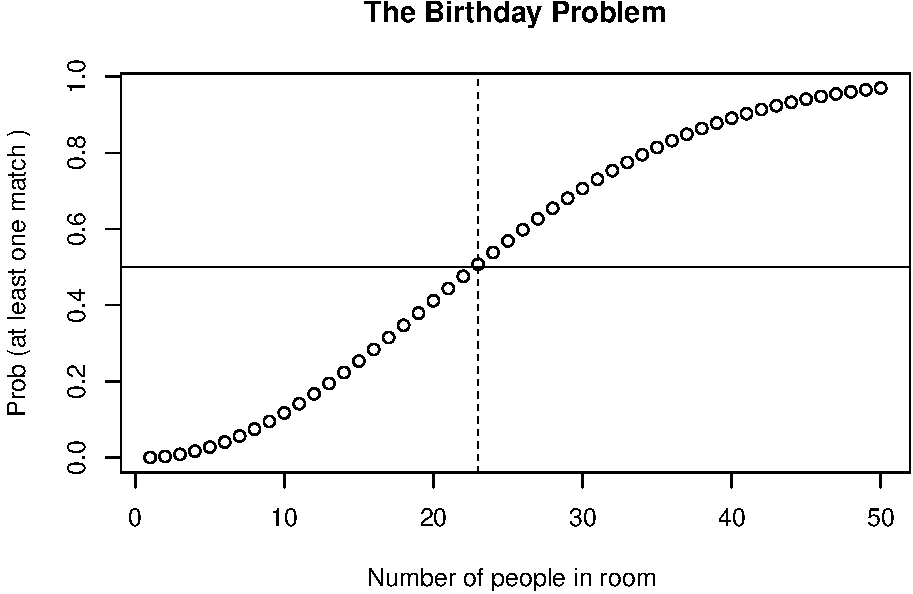
\includegraphics{probability_files/figure-latex/unnamed-chunk-6-1.pdf}

或者可以自己写计算概率的函数:

\begin{Shaded}
\begin{Highlighting}[]
\NormalTok{prob.birth<-function(n)}
  \NormalTok{\{if( n<}\StringTok{ }\DecValTok{365}\NormalTok{) }
    \KeywordTok{return}\NormalTok{(}\DecValTok{1}\NormalTok{-}\KeywordTok{choose}\NormalTok{(}\DecValTok{365}\NormalTok{,n)*}\KeywordTok{factorial}\NormalTok{(n)/}\DecValTok{365}\NormalTok{^n)}
  \NormalTok{else}
    \KeywordTok{return}\NormalTok{(}\DecValTok{1}\NormalTok{)}
  \NormalTok{\}}

\NormalTok{g2 <-}\StringTok{ }\KeywordTok{sapply}\NormalTok{(}\DecValTok{1}\NormalTok{:}\DecValTok{50}\NormalTok{, prob.birth)}
\KeywordTok{plot} \NormalTok{(}\DecValTok{1}\NormalTok{:}\DecValTok{50} \NormalTok{, g2,}
      \DataTypeTok{xlab =} \StringTok{"Number of people in room "}\NormalTok{,}
      \DataTypeTok{ylab =} \StringTok{"Prob (at least one match )"}\NormalTok{,}
      \DataTypeTok{main =} \StringTok{"The Birthday Problem"}\NormalTok{)}
\KeywordTok{abline} \NormalTok{(}\DataTypeTok{h =} \FloatTok{0.5}\NormalTok{)}
\KeywordTok{abline} \NormalTok{(}\DataTypeTok{v =} \DecValTok{23}\NormalTok{, }\DataTypeTok{lty =} \DecValTok{2}\NormalTok{) }\CommentTok{# 虚线}
\end{Highlighting}
\end{Shaded}

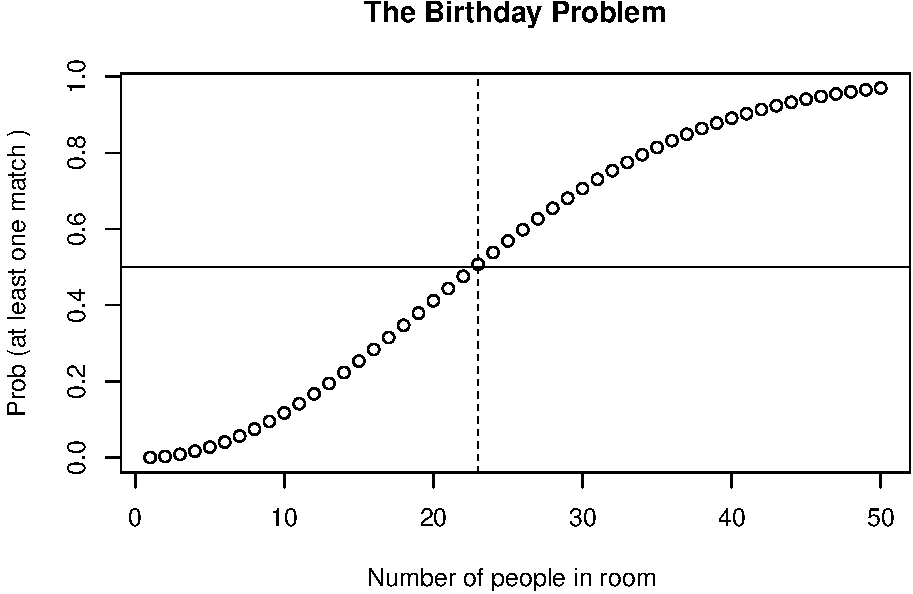
\includegraphics{probability_files/figure-latex/unnamed-chunk-7-1.pdf}

如果你要计算至少有一个人和你生日相同的概率:

\begin{Shaded}
\begin{Highlighting}[]
\NormalTok{q.birth<-function(n)\{}\KeywordTok{return}\NormalTok{(}\DecValTok{1}\NormalTok{-(}\DecValTok{364}\NormalTok{/}\DecValTok{365}\NormalTok{)^n)\}}
\NormalTok{x <-}\StringTok{ }\DecValTok{0}\NormalTok{:}\DecValTok{50}
\NormalTok{z <-}\StringTok{ }\OtherTok{NULL}
\NormalTok{for(i in }\DecValTok{1}\NormalTok{:}\KeywordTok{length}\NormalTok{(x))z[i]<-}\KeywordTok{q.birth}\NormalTok{(x[i])}
\KeywordTok{plot}\NormalTok{(x,z,}
     \DataTypeTok{xlab =} \StringTok{"Number of people in room "}\NormalTok{,}
     \DataTypeTok{ylab =} \StringTok{"Prob (at least one match with you)"}\NormalTok{,}
     \DataTypeTok{main =} \StringTok{"The Birthday Problem"}\NormalTok{)}
\KeywordTok{points}\NormalTok{(x,z)}
\end{Highlighting}
\end{Shaded}

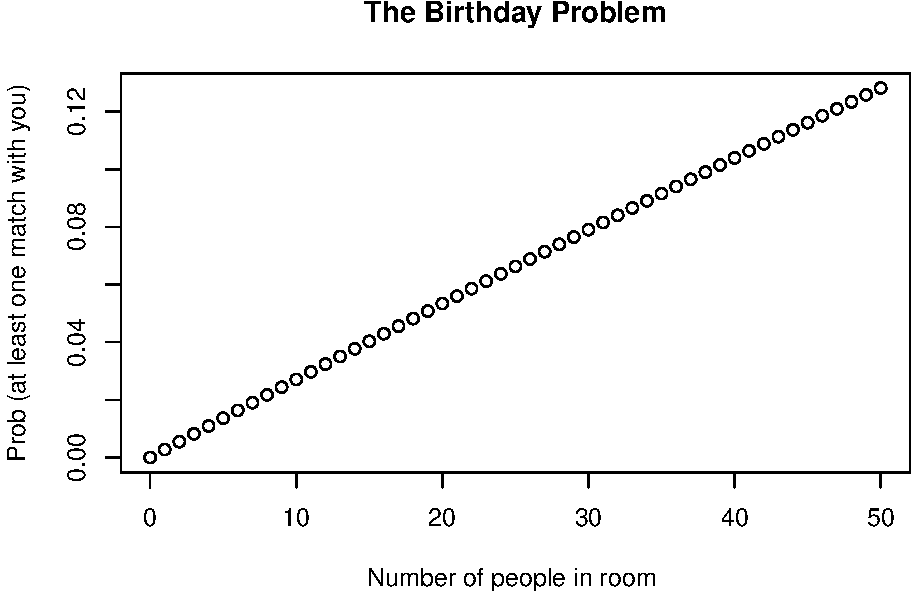
\includegraphics{probability_files/figure-latex/unnamed-chunk-8-1.pdf}

\textbf{Buffon投针试验}

\begin{Shaded}
\begin{Highlighting}[]
\CommentTok{# 绘制空白图形}
\KeywordTok{plot}\NormalTok{(}\KeywordTok{c}\NormalTok{(}\DecValTok{0}\NormalTok{,}\DecValTok{2}\NormalTok{),}\KeywordTok{c}\NormalTok{(}\DecValTok{0}\NormalTok{,}\DecValTok{2}\NormalTok{),}\DataTypeTok{type=}\StringTok{'n'}\NormalTok{,}\DataTypeTok{main=}\StringTok{'布丰投针实验'}\NormalTok{,}\DataTypeTok{xlab=}\StringTok{'X'}\NormalTok{,}\DataTypeTok{ylab=}\StringTok{'Y'}\NormalTok{)}
\end{Highlighting}
\end{Shaded}

\begin{verbatim}
## Warning in title(...): conversion failure on '布丰投针实验' in
## 'mbcsToSbcs': dot substituted for <e5>
\end{verbatim}

\begin{verbatim}
## Warning in title(...): conversion failure on '布丰投针实验' in
## 'mbcsToSbcs': dot substituted for <b8>
\end{verbatim}

\begin{verbatim}
## Warning in title(...): conversion failure on '布丰投针实验' in
## 'mbcsToSbcs': dot substituted for <83>
\end{verbatim}

\begin{verbatim}
## Warning in title(...): conversion failure on '布丰投针实验' in
## 'mbcsToSbcs': dot substituted for <e4>
\end{verbatim}

\begin{verbatim}
## Warning in title(...): conversion failure on '布丰投针实验' in
## 'mbcsToSbcs': dot substituted for <b8>
\end{verbatim}

\begin{verbatim}
## Warning in title(...): conversion failure on '布丰投针实验' in
## 'mbcsToSbcs': dot substituted for <b0>
\end{verbatim}

\begin{verbatim}
## Warning in title(...): conversion failure on '布丰投针实验' in
## 'mbcsToSbcs': dot substituted for <e6>
\end{verbatim}

\begin{verbatim}
## Warning in title(...): conversion failure on '布丰投针实验' in
## 'mbcsToSbcs': dot substituted for <8a>
\end{verbatim}

\begin{verbatim}
## Warning in title(...): conversion failure on '布丰投针实验' in
## 'mbcsToSbcs': dot substituted for <95>
\end{verbatim}

\begin{verbatim}
## Warning in title(...): conversion failure on '布丰投针实验' in
## 'mbcsToSbcs': dot substituted for <e9>
\end{verbatim}

\begin{verbatim}
## Warning in title(...): conversion failure on '布丰投针实验' in
## 'mbcsToSbcs': dot substituted for <92>
\end{verbatim}

\begin{verbatim}
## Warning in title(...): conversion failure on '布丰投针实验' in
## 'mbcsToSbcs': dot substituted for <88>
\end{verbatim}

\begin{verbatim}
## Warning in title(...): conversion failure on '布丰投针实验' in
## 'mbcsToSbcs': dot substituted for <e5>
\end{verbatim}

\begin{verbatim}
## Warning in title(...): conversion failure on '布丰投针实验' in
## 'mbcsToSbcs': dot substituted for <ae>
\end{verbatim}

\begin{verbatim}
## Warning in title(...): conversion failure on '布丰投针实验' in
## 'mbcsToSbcs': dot substituted for <9e>
\end{verbatim}

\begin{verbatim}
## Warning in title(...): conversion failure on '布丰投针实验' in
## 'mbcsToSbcs': dot substituted for <e9>
\end{verbatim}

\begin{verbatim}
## Warning in title(...): conversion failure on '布丰投针实验' in
## 'mbcsToSbcs': dot substituted for <aa>
\end{verbatim}

\begin{verbatim}
## Warning in title(...): conversion failure on '布丰投针实验' in
## 'mbcsToSbcs': dot substituted for <8c>
\end{verbatim}

\begin{Shaded}
\begin{Highlighting}[]
\CommentTok{# 增加平行线}
\KeywordTok{abline}\NormalTok{(}\DataTypeTok{h=}\FloatTok{0.5}\NormalTok{)}
\KeywordTok{abline}\NormalTok{(}\DataTypeTok{h=}\FloatTok{1.5}\NormalTok{,}\DataTypeTok{col=}\StringTok{'red'}\NormalTok{)}
\NormalTok{finished <-}\StringTok{ }\OtherTok{FALSE}
\CommentTok{# trial为实验次数,cross为交叉次数}
\NormalTok{trial <-}\StringTok{ }\DecValTok{0}
\NormalTok{cross <-}\StringTok{ }\DecValTok{0}
\NormalTok{for(i in }\DecValTok{1}\NormalTok{:}\DecValTok{50}\NormalTok{)\{}
    \CommentTok{# Dist为针的中心距离红线的垂直距离}
    \CommentTok{# Theta为针的角度}
    \NormalTok{Dist <-}\StringTok{ }\KeywordTok{runif}\NormalTok{(}\DecValTok{1}\NormalTok{,}\DataTypeTok{min=}\DecValTok{0}\NormalTok{,}\DataTypeTok{max=}\DecValTok{1}\NormalTok{/}\DecValTok{2}\NormalTok{)}
    \NormalTok{Theta <-}\StringTok{ }\KeywordTok{runif}\NormalTok{(}\DecValTok{1}\NormalTok{,}\DecValTok{0}\NormalTok{,pi)}
    \CommentTok{# central.x为针中心点的横坐标}
    \CommentTok{# central.y为针中心点的纵坐标}
    \NormalTok{central.x <-}\StringTok{ }\KeywordTok{runif}\NormalTok{(}\DecValTok{1}\NormalTok{,}\FloatTok{0.5}\NormalTok{,}\FloatTok{1.5}\NormalTok{)}
    \NormalTok{central.y <-}\StringTok{ }\NormalTok{Dist +}\DecValTok{1}
    \CommentTok{# 计算针两端的坐标}
    \NormalTok{y1 <-}\StringTok{ }\KeywordTok{sin}\NormalTok{(Theta)/}\DecValTok{4} \NormalTok{+}\StringTok{ }\NormalTok{central.y}
    \NormalTok{x1 <-}\StringTok{ }\KeywordTok{cos}\NormalTok{(Theta)/}\DecValTok{4} \NormalTok{+}\StringTok{ }\NormalTok{central.x}
    \NormalTok{y2 <-}\StringTok{ }\KeywordTok{sin}\NormalTok{(Theta+pi)/}\DecValTok{4} \NormalTok{+}\StringTok{ }\NormalTok{central.y}
    \NormalTok{x2 <-}\StringTok{ }\KeywordTok{cos}\NormalTok{(Theta+pi)/}\DecValTok{4} \NormalTok{+}\StringTok{ }\NormalTok{central.x}
    \NormalTok{trial <-}\StringTok{ }\NormalTok{trial +}\DecValTok{1}
    \CommentTok{# 计数交叉次数}
    \NormalTok{cross <-}\StringTok{ }\NormalTok{cross +}\StringTok{ }\KeywordTok{ifelse}\NormalTok{(}\FloatTok{0.25}\NormalTok{*}\KeywordTok{sin}\NormalTok{(Theta)>=Dist,}\DecValTok{1}\NormalTok{,}\DecValTok{0}\NormalTok{)}
    \CommentTok{# 绘制针的线型和中心点}
    \KeywordTok{lines}\NormalTok{(}\KeywordTok{c}\NormalTok{(x1,x2),}\KeywordTok{c}\NormalTok{(y1,y2),}\DataTypeTok{lty=}\DecValTok{2}\NormalTok{)}
    \KeywordTok{points}\NormalTok{(central.x,central.y,}\DataTypeTok{pch=}\DecValTok{16}\NormalTok{,}\DataTypeTok{col=}\StringTok{'grey'}\NormalTok{)}
    \KeywordTok{cat}\NormalTok{(}\StringTok{'trial='}\NormalTok{,trial,}\StringTok{'cross='}\NormalTok{,cross,}\StringTok{'PI='}\NormalTok{,trial/cross,}\StringTok{'}\CharTok{\textbackslash{}n}\StringTok{'}\NormalTok{)}
\NormalTok{\}}
\end{Highlighting}
\end{Shaded}

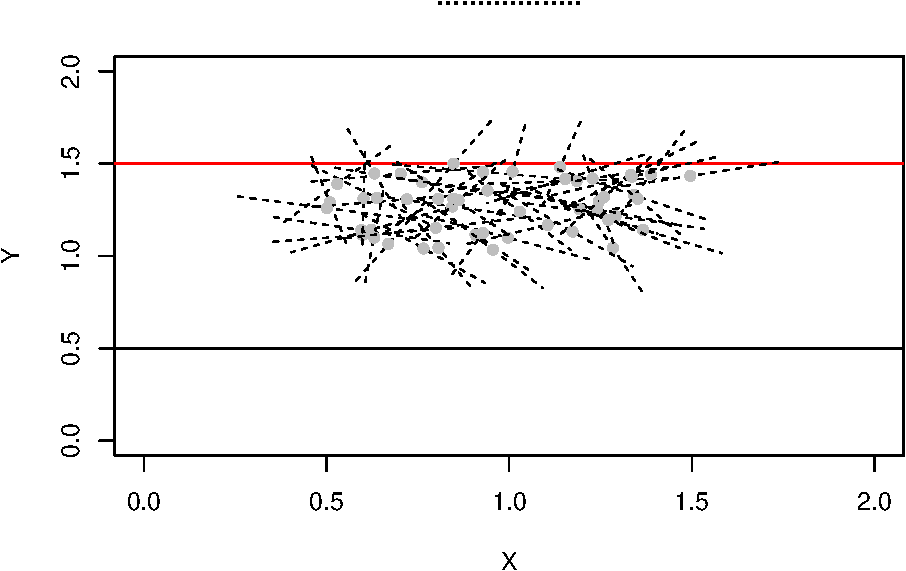
\includegraphics{probability_files/figure-latex/unnamed-chunk-9-1.pdf}

\begin{verbatim}
## trial= 1 cross= 0 PI= Inf 
## trial= 2 cross= 1 PI= 2 
## trial= 3 cross= 1 PI= 3 
## trial= 4 cross= 2 PI= 2 
## trial= 5 cross= 2 PI= 2.5 
## trial= 6 cross= 3 PI= 2 
## trial= 7 cross= 3 PI= 2.333333 
## trial= 8 cross= 3 PI= 2.666667 
## trial= 9 cross= 3 PI= 3 
## trial= 10 cross= 3 PI= 3.333333 
## trial= 11 cross= 3 PI= 3.666667 
## trial= 12 cross= 3 PI= 4 
## trial= 13 cross= 3 PI= 4.333333 
## trial= 14 cross= 3 PI= 4.666667 
## trial= 15 cross= 3 PI= 5 
## trial= 16 cross= 3 PI= 5.333333 
## trial= 17 cross= 3 PI= 5.666667 
## trial= 18 cross= 3 PI= 6 
## trial= 19 cross= 3 PI= 6.333333 
## trial= 20 cross= 3 PI= 6.666667 
## trial= 21 cross= 4 PI= 5.25 
## trial= 22 cross= 4 PI= 5.5 
## trial= 23 cross= 5 PI= 4.6 
## trial= 24 cross= 5 PI= 4.8 
## trial= 25 cross= 5 PI= 5 
## trial= 26 cross= 6 PI= 4.333333 
## trial= 27 cross= 6 PI= 4.5 
## trial= 28 cross= 6 PI= 4.666667 
## trial= 29 cross= 6 PI= 4.833333 
## trial= 30 cross= 6 PI= 5 
## trial= 31 cross= 7 PI= 4.428571 
## trial= 32 cross= 8 PI= 4 
## trial= 33 cross= 8 PI= 4.125 
## trial= 34 cross= 9 PI= 3.777778 
## trial= 35 cross= 9 PI= 3.888889 
## trial= 36 cross= 9 PI= 4 
## trial= 37 cross= 9 PI= 4.111111 
## trial= 38 cross= 9 PI= 4.222222 
## trial= 39 cross= 9 PI= 4.333333 
## trial= 40 cross= 9 PI= 4.444444 
## trial= 41 cross= 10 PI= 4.1 
## trial= 42 cross= 10 PI= 4.2 
## trial= 43 cross= 10 PI= 4.3 
## trial= 44 cross= 10 PI= 4.4 
## trial= 45 cross= 10 PI= 4.5 
## trial= 46 cross= 10 PI= 4.6 
## trial= 47 cross= 10 PI= 4.7 
## trial= 48 cross= 10 PI= 4.8 
## trial= 49 cross= 10 PI= 4.9 
## trial= 50 cross= 10 PI= 5
\end{verbatim}

\subsubsection{条件概率}

\begin{Shaded}
\begin{Highlighting}[]
\NormalTok{S3 <-}\StringTok{ }\KeywordTok{rolldie}\NormalTok{(}\DecValTok{2}\NormalTok{, }\DataTypeTok{makespace =} \OtherTok{TRUE}\NormalTok{) }\CommentTok{# assumes ELM}
\KeywordTok{head}\NormalTok{(S3)}
\end{Highlighting}
\end{Shaded}

\begin{verbatim}
##   X1 X2      probs
## 1  1  1 0.02777778
## 2  2  1 0.02777778
## 3  3  1 0.02777778
## 4  4  1 0.02777778
## 5  5  1 0.02777778
## 6  6  1 0.02777778
\end{verbatim}

\begin{Shaded}
\begin{Highlighting}[]
\NormalTok{A <-}\StringTok{ }\KeywordTok{subset}\NormalTok{(S3, X1 ==}\StringTok{ }\NormalTok{X2)}
\NormalTok{B <-}\StringTok{ }\KeywordTok{subset}\NormalTok{(S3, X1 +}\StringTok{ }\NormalTok{X2 >=}\StringTok{ }\DecValTok{8}\NormalTok{)}
\KeywordTok{prob}\NormalTok{(A,}\DataTypeTok{given=}\NormalTok{B) }\CommentTok{# B的条件下求A的概率}
\end{Highlighting}
\end{Shaded}

\begin{verbatim}
## 'prob' is deprecated; use 'Prob' instead.
\end{verbatim}

\begin{verbatim}
## [1] 0.2
\end{verbatim}

\begin{Shaded}
\begin{Highlighting}[]
\KeywordTok{prob}\NormalTok{(S3,X1==X2, }\DataTypeTok{given=}\NormalTok{(X1+X2>=}\DecValTok{8}\NormalTok{)) }\CommentTok{# X1+X2>=8的条件下求A的概率}
\end{Highlighting}
\end{Shaded}

\begin{verbatim}
## 'prob' is deprecated; use 'Prob' instead.
\end{verbatim}

\begin{verbatim}
## [1] 0.2
\end{verbatim}

\subsection{二、随机变量及其分布}

\subsubsection{离散型随机变量}

\textbf{二项分布}

\begin{Shaded}
\begin{Highlighting}[]
\KeywordTok{dbinom}\NormalTok{(}\DataTypeTok{x=}\DecValTok{2}\NormalTok{,}\DataTypeTok{size=}\DecValTok{20}\NormalTok{,}\DataTypeTok{prob=}\FloatTok{0.5}\NormalTok{)}
\end{Highlighting}
\end{Shaded}

\begin{verbatim}
## [1] 0.0001811981
\end{verbatim}

\begin{Shaded}
\begin{Highlighting}[]
\KeywordTok{pbinom}\NormalTok{(}\DataTypeTok{q=}\DecValTok{2}\NormalTok{,}\DataTypeTok{size=}\DecValTok{20}\NormalTok{,}\DataTypeTok{prob=}\FloatTok{0.5}\NormalTok{)}
\end{Highlighting}
\end{Shaded}

\begin{verbatim}
## [1] 0.0002012253
\end{verbatim}

\begin{Shaded}
\begin{Highlighting}[]
\KeywordTok{qbinom}\NormalTok{(}\DataTypeTok{p=}\FloatTok{0.4}\NormalTok{,}\DataTypeTok{size=}\DecValTok{20}\NormalTok{,}\DataTypeTok{prob=}\FloatTok{0.5}\NormalTok{)}
\end{Highlighting}
\end{Shaded}

\begin{verbatim}
## [1] 9
\end{verbatim}

\begin{Shaded}
\begin{Highlighting}[]
\KeywordTok{rbinom}\NormalTok{(}\DataTypeTok{n=}\DecValTok{5}\NormalTok{,}\DataTypeTok{size=}\DecValTok{20}\NormalTok{,}\DataTypeTok{prob=}\FloatTok{0.5}\NormalTok{)}
\end{Highlighting}
\end{Shaded}

\begin{verbatim}
## [1] 12 10  9  8 11
\end{verbatim}

\begin{Shaded}
\begin{Highlighting}[]
\KeywordTok{plot}\NormalTok{(}\KeywordTok{dbinom}\NormalTok{(}\DecValTok{0}\NormalTok{:}\DecValTok{20}\NormalTok{,}\DataTypeTok{size=}\DecValTok{20}\NormalTok{,}\DataTypeTok{prob=}\FloatTok{0.5}\NormalTok{),}\DataTypeTok{type=}\StringTok{"h"}\NormalTok{)}
\end{Highlighting}
\end{Shaded}

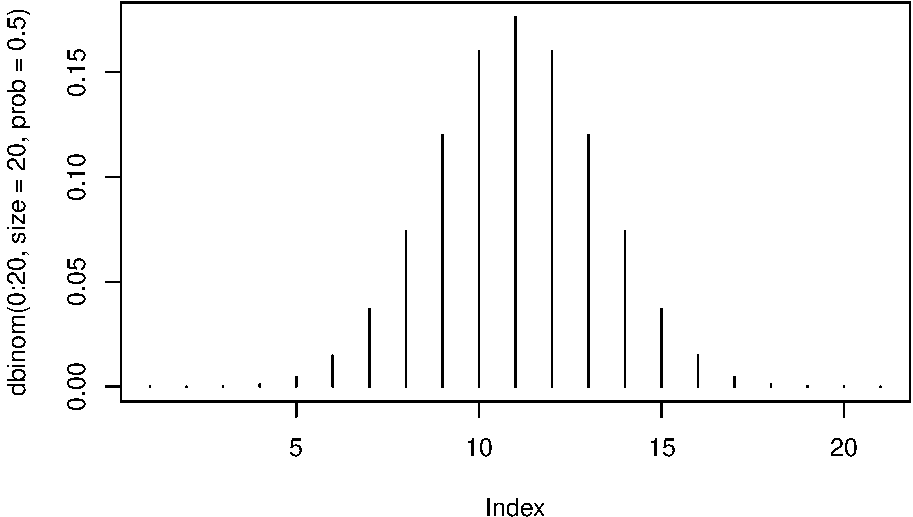
\includegraphics{probability_files/figure-latex/unnamed-chunk-11-1.pdf}

\begin{Shaded}
\begin{Highlighting}[]
\KeywordTok{plot}\NormalTok{(}\KeywordTok{dbinom}\NormalTok{(}\DecValTok{0}\NormalTok{:}\DecValTok{20}\NormalTok{,}\DataTypeTok{size=}\DecValTok{20}\NormalTok{,}\DataTypeTok{prob=}\FloatTok{0.8}\NormalTok{),}\DataTypeTok{type=}\StringTok{"h"}\NormalTok{)}
\end{Highlighting}
\end{Shaded}

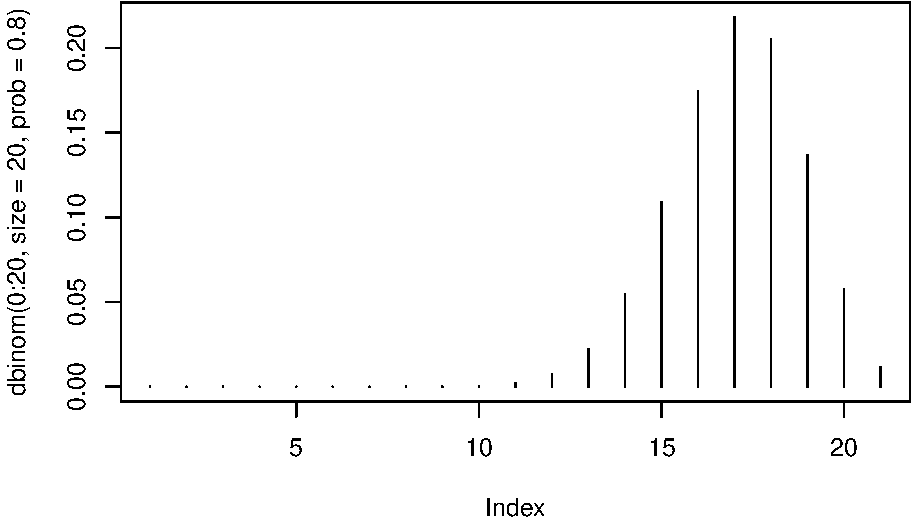
\includegraphics{probability_files/figure-latex/unnamed-chunk-11-2.pdf}

\textbf{超几何分布}

\begin{Shaded}
\begin{Highlighting}[]
\KeywordTok{dhyper}\NormalTok{(}\DataTypeTok{x=}\DecValTok{2}\NormalTok{, }\DataTypeTok{m=}\DecValTok{10}\NormalTok{, }\DataTypeTok{n=}\DecValTok{30}\NormalTok{, }\DataTypeTok{k=}\DecValTok{6}\NormalTok{)}
\end{Highlighting}
\end{Shaded}

\begin{verbatim}
## [1] 0.3212879
\end{verbatim}

\begin{Shaded}
\begin{Highlighting}[]
\KeywordTok{phyper}\NormalTok{(}\DataTypeTok{q=}\DecValTok{2}\NormalTok{, }\DataTypeTok{m=}\DecValTok{10}\NormalTok{, }\DataTypeTok{n=}\DecValTok{30}\NormalTok{, }\DataTypeTok{k=}\DecValTok{6}\NormalTok{)}
\end{Highlighting}
\end{Shaded}

\begin{verbatim}
## [1] 0.8472481
\end{verbatim}

\begin{Shaded}
\begin{Highlighting}[]
\KeywordTok{qhyper}\NormalTok{(}\FloatTok{0.3}\NormalTok{, }\DataTypeTok{m=}\DecValTok{10}\NormalTok{, }\DataTypeTok{n=}\DecValTok{30}\NormalTok{, }\DataTypeTok{k=}\DecValTok{6}\NormalTok{)}
\end{Highlighting}
\end{Shaded}

\begin{verbatim}
## [1] 1
\end{verbatim}

\begin{Shaded}
\begin{Highlighting}[]
\KeywordTok{rhyper}\NormalTok{(}\DataTypeTok{nn=}\DecValTok{10}\NormalTok{, }\DataTypeTok{m=}\DecValTok{10}\NormalTok{, }\DataTypeTok{n=}\DecValTok{30}\NormalTok{, }\DataTypeTok{k=}\DecValTok{6}\NormalTok{)}
\end{Highlighting}
\end{Shaded}

\begin{verbatim}
##  [1] 2 2 3 2 2 1 3 1 1 1
\end{verbatim}

\textbf{几何分布}

\begin{Shaded}
\begin{Highlighting}[]
\KeywordTok{dgeom}\NormalTok{(}\DecValTok{4}\NormalTok{,}\DataTypeTok{prob=}\FloatTok{0.8}\NormalTok{)}
\end{Highlighting}
\end{Shaded}

\begin{verbatim}
## [1] 0.00128
\end{verbatim}

\begin{Shaded}
\begin{Highlighting}[]
\KeywordTok{pgeom}\NormalTok{(}\DecValTok{4}\NormalTok{, }\DataTypeTok{prob =} \FloatTok{0.8}\NormalTok{)}
\end{Highlighting}
\end{Shaded}

\begin{verbatim}
## [1] 0.99968
\end{verbatim}

\begin{Shaded}
\begin{Highlighting}[]
\KeywordTok{qgeom}\NormalTok{(}\FloatTok{0.4}\NormalTok{,}\DataTypeTok{prob=}\FloatTok{0.8}\NormalTok{)}
\end{Highlighting}
\end{Shaded}

\begin{verbatim}
## [1] 0
\end{verbatim}

\begin{Shaded}
\begin{Highlighting}[]
\KeywordTok{rgeom}\NormalTok{(}\DecValTok{10}\NormalTok{,}\DataTypeTok{prob=}\FloatTok{0.8}\NormalTok{)}
\end{Highlighting}
\end{Shaded}

\begin{verbatim}
##  [1] 1 0 0 0 0 0 2 0 0 0
\end{verbatim}

\begin{Shaded}
\begin{Highlighting}[]
\KeywordTok{plot}\NormalTok{(}\KeywordTok{dgeom}\NormalTok{(}\DecValTok{0}\NormalTok{:}\DecValTok{20}\NormalTok{,}\DataTypeTok{prob=}\FloatTok{0.5}\NormalTok{),}\DataTypeTok{type=}\StringTok{"h"}\NormalTok{)}
\end{Highlighting}
\end{Shaded}

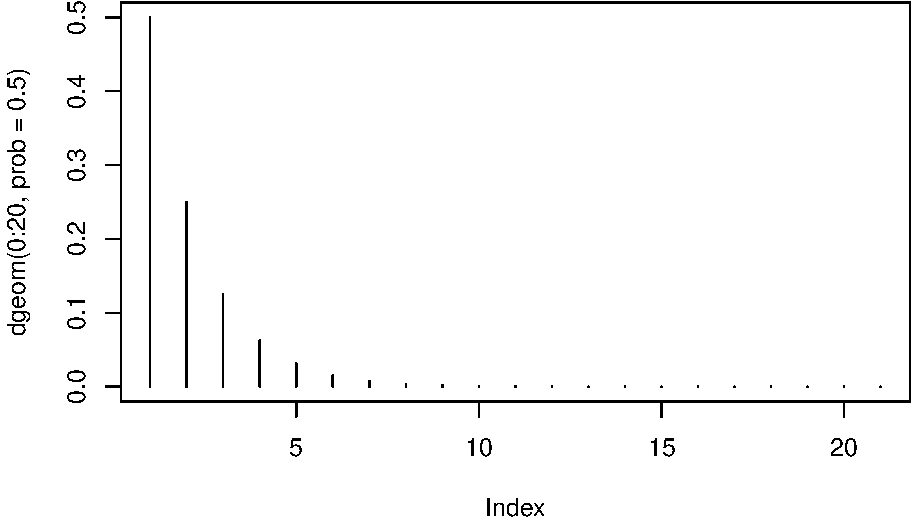
\includegraphics{probability_files/figure-latex/unnamed-chunk-13-1.pdf}

\begin{Shaded}
\begin{Highlighting}[]
\KeywordTok{plot}\NormalTok{(}\KeywordTok{dgeom}\NormalTok{(}\DecValTok{0}\NormalTok{:}\DecValTok{20}\NormalTok{,}\DataTypeTok{prob=}\FloatTok{0.8}\NormalTok{),}\DataTypeTok{type=}\StringTok{"h"}\NormalTok{)}
\end{Highlighting}
\end{Shaded}

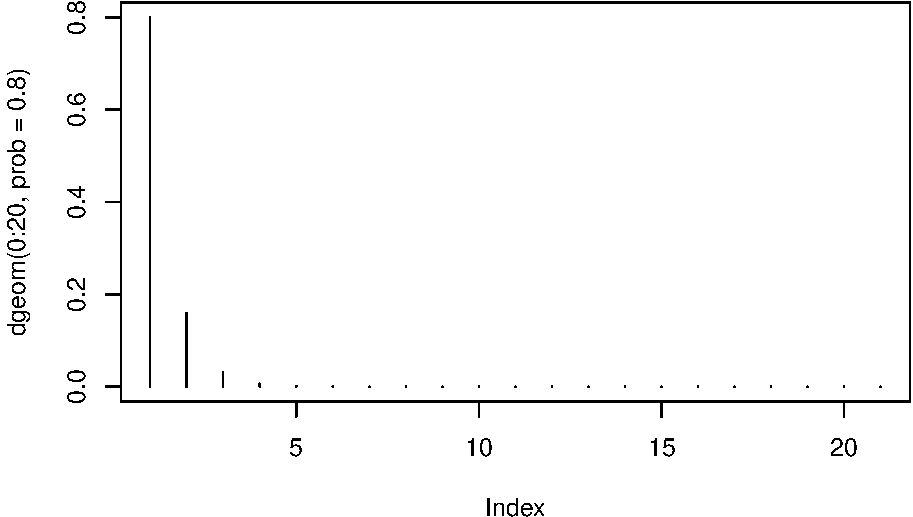
\includegraphics{probability_files/figure-latex/unnamed-chunk-13-2.pdf}

\textbf{负二项分布}

\begin{Shaded}
\begin{Highlighting}[]
\KeywordTok{dnbinom}\NormalTok{(}\DataTypeTok{x=}\DecValTok{5}\NormalTok{,}\DataTypeTok{size=}\DecValTok{3}\NormalTok{,}\DataTypeTok{prob=}\FloatTok{0.4}\NormalTok{)   }
\end{Highlighting}
\end{Shaded}

\begin{verbatim}
## [1] 0.1045094
\end{verbatim}

\begin{Shaded}
\begin{Highlighting}[]
\KeywordTok{pnbinom}\NormalTok{(}\DecValTok{5}\NormalTok{,}\DataTypeTok{size=}\DecValTok{3}\NormalTok{,}\DataTypeTok{prob=}\FloatTok{0.4}\NormalTok{)}
\end{Highlighting}
\end{Shaded}

\begin{verbatim}
## [1] 0.6846054
\end{verbatim}

\begin{Shaded}
\begin{Highlighting}[]
\KeywordTok{qnbinom}\NormalTok{(}\FloatTok{0.5}\NormalTok{,}\DataTypeTok{size=}\DecValTok{3}\NormalTok{,}\DataTypeTok{prob=}\FloatTok{0.4}\NormalTok{)}
\end{Highlighting}
\end{Shaded}

\begin{verbatim}
## [1] 4
\end{verbatim}

\begin{Shaded}
\begin{Highlighting}[]
\KeywordTok{rnbinom}\NormalTok{(}\DataTypeTok{n=}\DecValTok{10}\NormalTok{,}\DataTypeTok{size=}\DecValTok{3}\NormalTok{,}\DataTypeTok{prob=}\FloatTok{0.4}\NormalTok{)}
\end{Highlighting}
\end{Shaded}

\begin{verbatim}
##  [1] 5 2 2 5 1 7 5 8 2 1
\end{verbatim}

\begin{Shaded}
\begin{Highlighting}[]
\KeywordTok{plot}\NormalTok{(}\KeywordTok{dnbinom}\NormalTok{(}\DecValTok{0}\NormalTok{:}\DecValTok{20}\NormalTok{,}\DataTypeTok{size=}\DecValTok{5}\NormalTok{,}\DataTypeTok{p=}\FloatTok{0.5}\NormalTok{),}\DataTypeTok{type=}\StringTok{"h"}\NormalTok{)}
\end{Highlighting}
\end{Shaded}

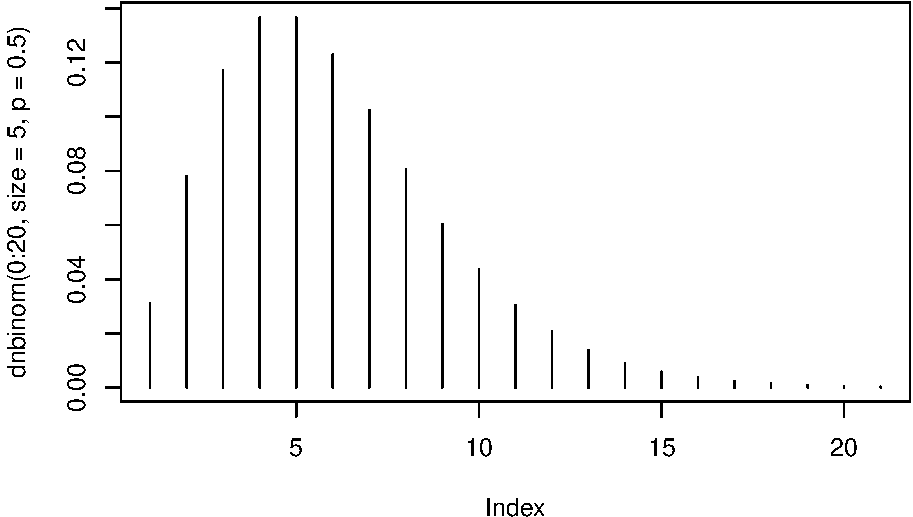
\includegraphics{probability_files/figure-latex/unnamed-chunk-14-1.pdf}

\textbf{泊松分布}

\begin{Shaded}
\begin{Highlighting}[]
\KeywordTok{dpois}\NormalTok{(}\DataTypeTok{x=}\DecValTok{0}\NormalTok{,}\DataTypeTok{lambda=}\FloatTok{2.4}\NormalTok{)}
\end{Highlighting}
\end{Shaded}

\begin{verbatim}
## [1] 0.09071795
\end{verbatim}

\begin{Shaded}
\begin{Highlighting}[]
\KeywordTok{ppois}\NormalTok{(}\DataTypeTok{q=}\DecValTok{10}\NormalTok{,}\DataTypeTok{lambda=}\FloatTok{2.4}\NormalTok{)}
\end{Highlighting}
\end{Shaded}

\begin{verbatim}
## [1] 0.999957
\end{verbatim}

\begin{Shaded}
\begin{Highlighting}[]
\KeywordTok{qpois}\NormalTok{(}\DataTypeTok{p=}\FloatTok{0.9}\NormalTok{,}\DataTypeTok{lambda=}\FloatTok{2.4}\NormalTok{)}
\end{Highlighting}
\end{Shaded}

\begin{verbatim}
## [1] 4
\end{verbatim}

\begin{Shaded}
\begin{Highlighting}[]
\KeywordTok{rpois}\NormalTok{(}\DataTypeTok{n=}\DecValTok{10}\NormalTok{,}\DataTypeTok{lambda=}\FloatTok{2.4}\NormalTok{)}
\end{Highlighting}
\end{Shaded}

\begin{verbatim}
##  [1] 2 6 4 2 3 3 2 6 1 8
\end{verbatim}

\begin{Shaded}
\begin{Highlighting}[]
\KeywordTok{plot}\NormalTok{(}\KeywordTok{dpois}\NormalTok{(}\DecValTok{0}\NormalTok{:}\DecValTok{20}\NormalTok{,}\DataTypeTok{lambda=}\DecValTok{1}\NormalTok{),}\DataTypeTok{type=}\StringTok{"h"}\NormalTok{)}
\end{Highlighting}
\end{Shaded}

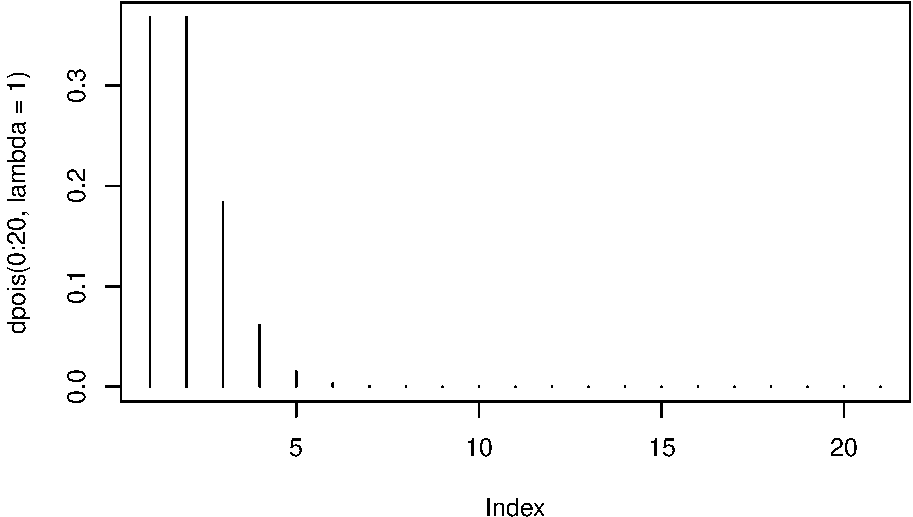
\includegraphics{probability_files/figure-latex/unnamed-chunk-15-1.pdf}

\begin{Shaded}
\begin{Highlighting}[]
\NormalTok{x <-}\StringTok{ }\DecValTok{0}\NormalTok{:}\DecValTok{20}
\KeywordTok{plot}\NormalTok{(x, }\KeywordTok{ppois}\NormalTok{(x, }\DecValTok{1}\NormalTok{), }\DataTypeTok{type=}\StringTok{"s"}\NormalTok{, }\DataTypeTok{lty=}\DecValTok{1}\NormalTok{,}\DataTypeTok{ylab=}\StringTok{"F(x)"}\NormalTok{, }\DataTypeTok{main=}\StringTok{"Poisson approx of binomial"}\NormalTok{)}
\KeywordTok{lines}\NormalTok{(x, }\KeywordTok{pbinom}\NormalTok{(x, }\DecValTok{100}\NormalTok{, }\FloatTok{0.01}\NormalTok{),}\DataTypeTok{type=}\StringTok{"s"}\NormalTok{,}\DataTypeTok{col=}\DecValTok{2}\NormalTok{,}\DataTypeTok{lty=}\DecValTok{2}\NormalTok{)}
\KeywordTok{legend}\NormalTok{(}\StringTok{"bottomright"}\NormalTok{,}\DataTypeTok{legend=}\KeywordTok{c}\NormalTok{(}\StringTok{"Poisson"}\NormalTok{,}\StringTok{"Binomial"}\NormalTok{),}\DataTypeTok{lty=}\DecValTok{1}\NormalTok{:}\DecValTok{2}\NormalTok{,}\DataTypeTok{col=}\DecValTok{1}\NormalTok{:}\DecValTok{2}\NormalTok{)}
\end{Highlighting}
\end{Shaded}

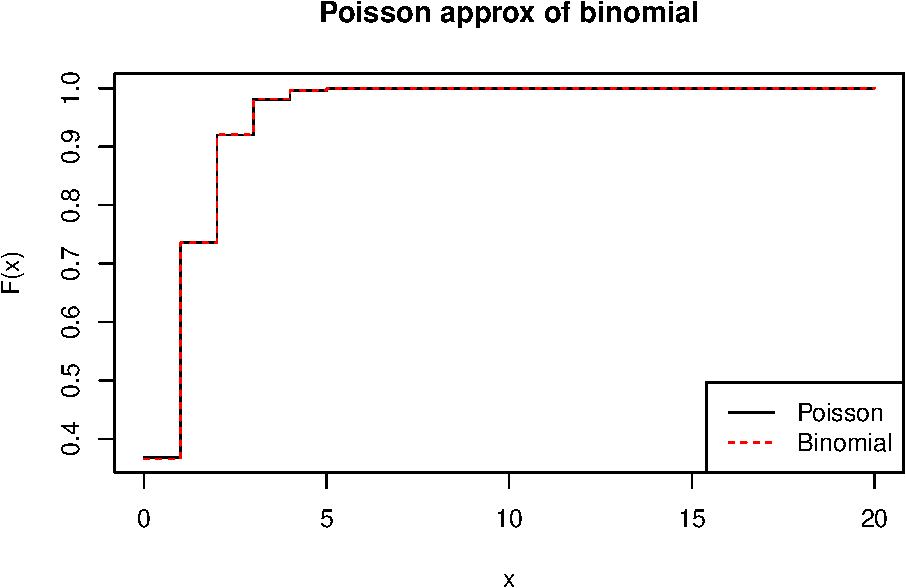
\includegraphics{probability_files/figure-latex/unnamed-chunk-15-2.pdf}

\textbf{二项分布的泊松近似和正态近似}

\begin{Shaded}
\begin{Highlighting}[]
\CommentTok{#P(X<=k)=pbinom(k,n,p)}
\CommentTok{#Poisson approximation: P(X<=k) app ppois(k,np)}
\CommentTok{#Normal approximation: P(X<=k) app pnorm(k,np,npq)}

\NormalTok{apprx <-}\StringTok{ }\NormalTok{function(n, p, }\DataTypeTok{R =} \DecValTok{1000}\NormalTok{, }\DataTypeTok{k =} \DecValTok{6}\NormalTok{) \{}
  \NormalTok{trueval <-}\StringTok{ }\KeywordTok{pbinom}\NormalTok{(k, n, p) }\CommentTok{# true binomial probability}
  \NormalTok{prob.zcc <-}\StringTok{ }\NormalTok{prob.zncc <-}\StringTok{ }\NormalTok{prob.pois <-}\StringTok{ }\OtherTok{NULL}  
  \NormalTok{q <-}\StringTok{ }\DecValTok{1}\NormalTok{-p}
  \NormalTok{for (i in }\DecValTok{1}\NormalTok{:R) \{}
    \NormalTok{x <-}\StringTok{ }\KeywordTok{rnorm}\NormalTok{(n, n *}\StringTok{ }\NormalTok{p, }\KeywordTok{sqrt}\NormalTok{(n *}\StringTok{ }\NormalTok{p *}\StringTok{ }\NormalTok{q))}
    \NormalTok{z.cc <-}\StringTok{ }\NormalTok{((k +}\StringTok{ }\NormalTok{.}\DecValTok{5}\NormalTok{) -}\StringTok{ }\KeywordTok{mean}\NormalTok{(x))/}\KeywordTok{sd}\NormalTok{(x) }\CommentTok{# with cont. correction}
    \NormalTok{prob.zcc[i] <-}\StringTok{ }\KeywordTok{pnorm}\NormalTok{(z.cc)}
    \NormalTok{z.ncc <-}\StringTok{ }\NormalTok{(k -}\StringTok{ }\KeywordTok{mean}\NormalTok{(x))/}\KeywordTok{sd}\NormalTok{(x) }\CommentTok{# no cont. correction}
    \NormalTok{prob.zncc[i] <-}\StringTok{ }\KeywordTok{pnorm}\NormalTok{(z.ncc)    }
    \NormalTok{y <-}\StringTok{ }\KeywordTok{rpois}\NormalTok{(n, n *}\StringTok{ }\NormalTok{p)}
    \NormalTok{prob.pois[i] <-}\StringTok{ }\KeywordTok{length}\NormalTok{(y[y <=}\StringTok{ }\NormalTok{k])/n}
  \NormalTok{\}}
  \KeywordTok{list}\NormalTok{(}\DataTypeTok{prob.zcc =} \NormalTok{prob.zcc, }\DataTypeTok{prob.zncc =} \NormalTok{prob.zncc, }
       \DataTypeTok{prob.pois =} \NormalTok{prob.pois, }\DataTypeTok{trueval =} \NormalTok{trueval)}
\NormalTok{\}}

\NormalTok{R <-}\StringTok{ }\DecValTok{1000}
\KeywordTok{set.seed}\NormalTok{(}\DecValTok{10}\NormalTok{)}
\NormalTok{out <-}\StringTok{ }\KeywordTok{apprx}\NormalTok{(}\DataTypeTok{n =} \DecValTok{200}\NormalTok{, }\DataTypeTok{p =} \NormalTok{.}\DecValTok{03}\NormalTok{, }\DataTypeTok{k =} \DecValTok{6}\NormalTok{, }\DataTypeTok{R =} \DecValTok{1000}\NormalTok{)}
\CommentTok{# windows(6,5)}
\KeywordTok{plot}\NormalTok{(}\DecValTok{1}\NormalTok{:R, out$prob.pois, }\DataTypeTok{type =} \StringTok{"l"}\NormalTok{, }
     \DataTypeTok{col =} \StringTok{"green"}\NormalTok{, }\DataTypeTok{xlab =} \StringTok{"Runs"}\NormalTok{, }
     \DataTypeTok{main =} \KeywordTok{expression}\NormalTok{(}\KeywordTok{paste}\NormalTok{(}\StringTok{"Simulated Probabilities: "}\NormalTok{, }
                             \NormalTok{n==}\DecValTok{200}\NormalTok{, }\StringTok{", "}\NormalTok{, p==}\FloatTok{0.03}\NormalTok{, }\DataTypeTok{sep=}\StringTok{""}\NormalTok{)),}
     \DataTypeTok{ylab =} \StringTok{"Probability"}\NormalTok{, }\DataTypeTok{ylim =} \KeywordTok{c}\NormalTok{(.}\DecValTok{3}\NormalTok{, .}\DecValTok{7}\NormalTok{))}
\KeywordTok{abline}\NormalTok{(}\DataTypeTok{h =} \NormalTok{out$trueval, }\DataTypeTok{col=}\StringTok{"red"}\NormalTok{, }\DataTypeTok{lty=}\DecValTok{2}\NormalTok{)}
\KeywordTok{lines}\NormalTok{(}\DecValTok{1}\NormalTok{:R, out$prob.zcc, }\DataTypeTok{lty =} \DecValTok{1}\NormalTok{, }\DataTypeTok{col =} \StringTok{"purple"}\NormalTok{)}
\KeywordTok{lines}\NormalTok{(}\DecValTok{1}\NormalTok{:R, out$prob.zncc, }\DataTypeTok{lty =} \DecValTok{1}\NormalTok{, }\DataTypeTok{col =} \StringTok{"orange"}\NormalTok{)}
\KeywordTok{legend}\NormalTok{(}\StringTok{"bottomleft"}\NormalTok{, }
       \KeywordTok{c}\NormalTok{(}\StringTok{"Poisson"}\NormalTok{, }\StringTok{"Normal (with cc)"}\NormalTok{, }\StringTok{"Normal (w/o cc)"}\NormalTok{),}
       \DataTypeTok{lty =} \KeywordTok{c}\NormalTok{(}\DecValTok{1}\NormalTok{), }\DataTypeTok{col =} \KeywordTok{c}\NormalTok{(}\StringTok{"green"}\NormalTok{, }\StringTok{"purple"}\NormalTok{, }\StringTok{"orange"}\NormalTok{))}
\end{Highlighting}
\end{Shaded}

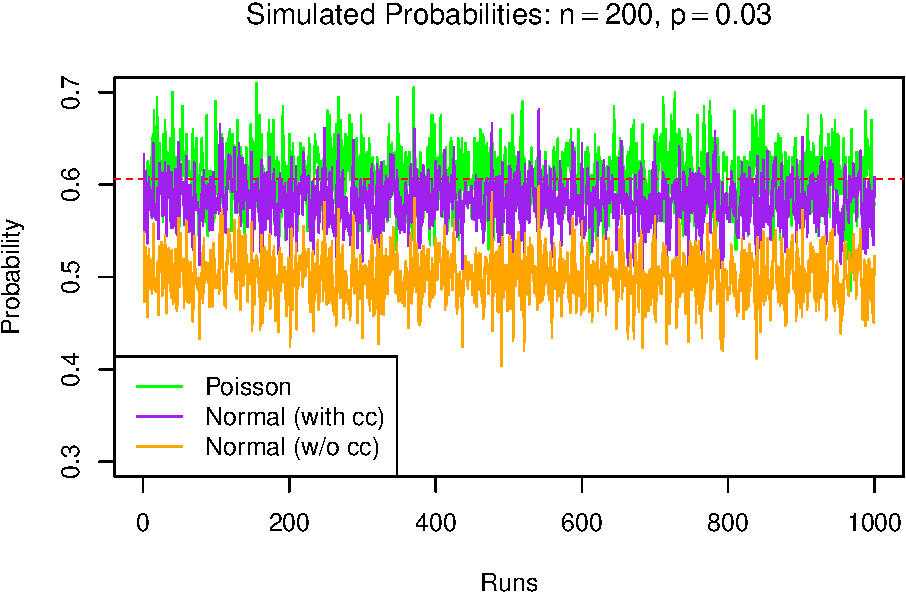
\includegraphics{probability_files/figure-latex/unnamed-chunk-16-1.pdf}

\begin{Shaded}
\begin{Highlighting}[]
\KeywordTok{set.seed}\NormalTok{(}\DecValTok{10}\NormalTok{)}
\NormalTok{out <-}\StringTok{ }\KeywordTok{apprx}\NormalTok{(}\DataTypeTok{n =} \DecValTok{200}\NormalTok{, }\DataTypeTok{p =} \NormalTok{.}\DecValTok{03}\NormalTok{, }\DataTypeTok{k =} \DecValTok{6}\NormalTok{, }\DataTypeTok{R =} \DecValTok{1000}\NormalTok{)}
\CommentTok{# windows(6,5)}
\KeywordTok{boxplot}\NormalTok{(out$prob.pois, }\DataTypeTok{boxwex =} \FloatTok{0.25}\NormalTok{, }\DataTypeTok{at =} \DecValTok{1}\NormalTok{:}\DecValTok{1} \NormalTok{-}\StringTok{ }\NormalTok{.}\DecValTok{25}\NormalTok{,}
        \DataTypeTok{col =} \StringTok{"green"}\NormalTok{,}
        \DataTypeTok{main =} \KeywordTok{expression}\NormalTok{(}\KeywordTok{paste}\NormalTok{(}\StringTok{"Approximating Binomial Probability: "}\NormalTok{, }
                                \NormalTok{n==}\DecValTok{200}\NormalTok{, }\StringTok{", "}\NormalTok{, p==}\FloatTok{0.03}\NormalTok{, }\DataTypeTok{sep=}\StringTok{""}\NormalTok{)),}
        \DataTypeTok{ylab =} \StringTok{"Probablity"}\NormalTok{, }
        \DataTypeTok{ylim =} \KeywordTok{c}\NormalTok{(out$trueval -}\StringTok{ }\FloatTok{0.2}\NormalTok{, out$trueval +}\StringTok{ }\FloatTok{0.25}\NormalTok{))}
\KeywordTok{boxplot}\NormalTok{(out$prob.zcc, }\DataTypeTok{boxwex =} \FloatTok{0.25}\NormalTok{, }\DataTypeTok{at =} \DecValTok{1}\NormalTok{:}\DecValTok{1} \NormalTok{+}\StringTok{ }\DecValTok{0}\NormalTok{, }\DataTypeTok{add =} \NormalTok{T,}
         \DataTypeTok{col =} \StringTok{"purple"}\NormalTok{)}
\KeywordTok{boxplot}\NormalTok{(out$prob.zncc, }\DataTypeTok{boxwex =} \FloatTok{0.25}\NormalTok{, }\DataTypeTok{at =} \DecValTok{1}\NormalTok{:}\DecValTok{1} \NormalTok{+}\StringTok{ }\FloatTok{0.25}\NormalTok{, }\DataTypeTok{add =} \NormalTok{T,}
         \DataTypeTok{col =} \StringTok{"orange"} \NormalTok{)}
\KeywordTok{abline}\NormalTok{(}\DataTypeTok{h =} \NormalTok{out$trueval, }\DataTypeTok{col =} \StringTok{"red"}\NormalTok{, }\DataTypeTok{lty=}\DecValTok{2}\NormalTok{)}
\KeywordTok{legend}\NormalTok{(}\StringTok{"topleft"}\NormalTok{, }\KeywordTok{c}\NormalTok{(}\StringTok{"Poisson"}\NormalTok{, }\StringTok{"Normal (with cc)"}\NormalTok{, }\StringTok{"Normal (w/o cc)"}\NormalTok{), }
           \DataTypeTok{fill =} \KeywordTok{c}\NormalTok{(}\StringTok{"green"}\NormalTok{, }\StringTok{"purple"}\NormalTok{, }\StringTok{"orange"}\NormalTok{))}
\end{Highlighting}
\end{Shaded}

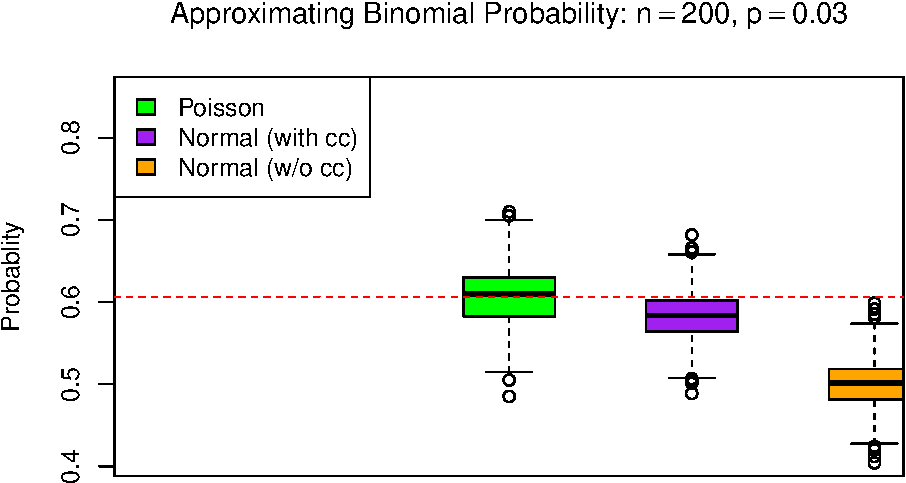
\includegraphics{probability_files/figure-latex/unnamed-chunk-16-2.pdf}

\subsubsection{连续型随机变量}

\textbf{正态分布}

\begin{Shaded}
\begin{Highlighting}[]
\KeywordTok{dnorm}\NormalTok{(}\DecValTok{0}\NormalTok{,}\DataTypeTok{mean=}\DecValTok{0}\NormalTok{,}\DataTypeTok{sd=}\DecValTok{1}\NormalTok{)}
\end{Highlighting}
\end{Shaded}

\begin{verbatim}
## [1] 0.3989423
\end{verbatim}

\begin{Shaded}
\begin{Highlighting}[]
\KeywordTok{pnorm}\NormalTok{(}\DecValTok{0}\NormalTok{)}
\end{Highlighting}
\end{Shaded}

\begin{verbatim}
## [1] 0.5
\end{verbatim}

\begin{Shaded}
\begin{Highlighting}[]
\KeywordTok{qnorm}\NormalTok{(}\FloatTok{2.5}\NormalTok{/}\DecValTok{100}\NormalTok{,}\DataTypeTok{lower.tail=}\NormalTok{F)}
\end{Highlighting}
\end{Shaded}

\begin{verbatim}
## [1] 1.959964
\end{verbatim}

\begin{Shaded}
\begin{Highlighting}[]
\KeywordTok{rnorm}\NormalTok{(}\DecValTok{10}\NormalTok{,}\DataTypeTok{mean=}\DecValTok{1}\NormalTok{,}\DataTypeTok{sd=}\FloatTok{1.5}\NormalTok{)}
\end{Highlighting}
\end{Shaded}

\begin{verbatim}
##  [1]  0.1963887 -0.4863110  1.4597941  0.9939968  0.6741421  1.5888671
##  [7]  0.6617092  2.2173455  1.1084923 -0.3535931
\end{verbatim}

\begin{Shaded}
\begin{Highlighting}[]
\CommentTok{# some plots}

\NormalTok{x <-}\StringTok{ }\KeywordTok{seq}\NormalTok{(-}\DecValTok{4}\NormalTok{, }\DecValTok{4}\NormalTok{, }\DataTypeTok{length =} \DecValTok{401}\NormalTok{)}
\KeywordTok{plot}\NormalTok{(x, }\KeywordTok{dnorm}\NormalTok{(x), }\DataTypeTok{type =} \StringTok{'l'}\NormalTok{) }\CommentTok{# N(0, 1)}
\CommentTok{# N(1, 1.5^2):}
\KeywordTok{lines}\NormalTok{(x, }\KeywordTok{dnorm}\NormalTok{(x, }\DataTypeTok{mean =} \DecValTok{1}\NormalTok{, }\DataTypeTok{sd =} \FloatTok{1.5}\NormalTok{), }\DataTypeTok{lty =} \StringTok{'dashed'}\NormalTok{)}
\end{Highlighting}
\end{Shaded}

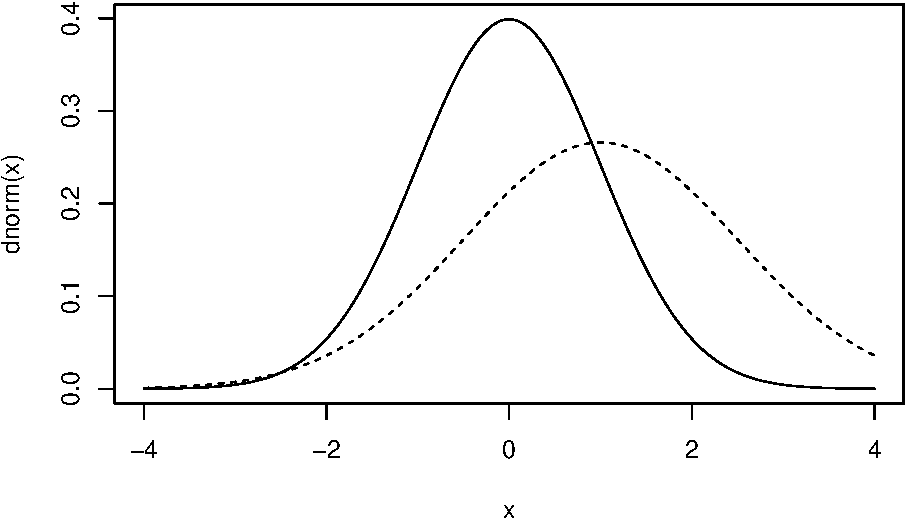
\includegraphics{probability_files/figure-latex/unnamed-chunk-17-1.pdf}

\begin{Shaded}
\begin{Highlighting}[]
\NormalTok{u <-}\StringTok{ }\KeywordTok{seq}\NormalTok{(}\DecValTok{0}\NormalTok{, }\DecValTok{1}\NormalTok{, }\DataTypeTok{length=}\DecValTok{401}\NormalTok{)}
\KeywordTok{plot}\NormalTok{(u, }\KeywordTok{qnorm}\NormalTok{(u), }\StringTok{'l'}\NormalTok{)}
\CommentTok{# lower.tail = FALSE gives q(1-u)}
\KeywordTok{lines}\NormalTok{(u, }\KeywordTok{qnorm}\NormalTok{(u, }\DataTypeTok{lower.tail =} \OtherTok{FALSE}\NormalTok{), }\DataTypeTok{lty =} \StringTok{'dashed'}\NormalTok{)}
\end{Highlighting}
\end{Shaded}

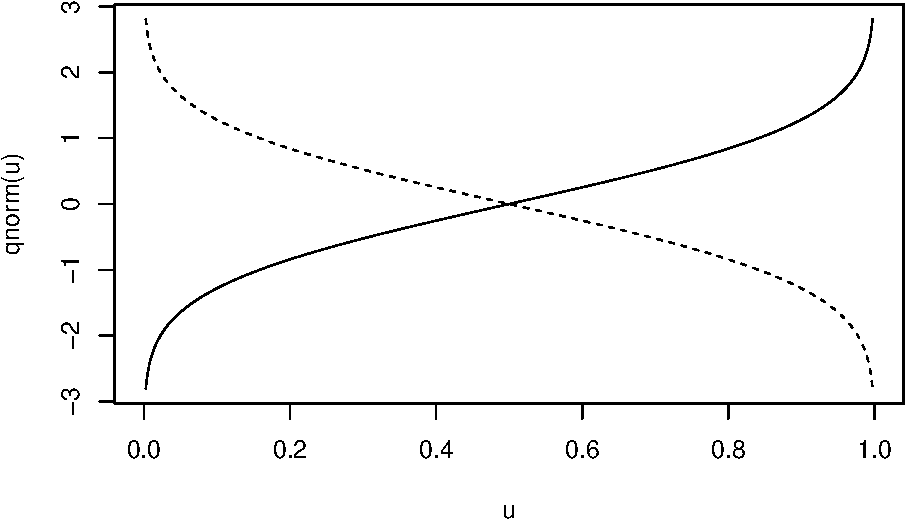
\includegraphics{probability_files/figure-latex/unnamed-chunk-17-2.pdf}

\begin{Shaded}
\begin{Highlighting}[]
\CommentTok{#cumulative distribution function}
\KeywordTok{curve}\NormalTok{(}\KeywordTok{pnorm}\NormalTok{(x), }\DataTypeTok{xlim=}\KeywordTok{c}\NormalTok{(-}\DecValTok{5}\NormalTok{,}\DecValTok{5}\NormalTok{), }\DataTypeTok{col=}\StringTok{'red'}\NormalTok{, }\DataTypeTok{lwd=}\DecValTok{3}\NormalTok{)}
\KeywordTok{title}\NormalTok{(}\DataTypeTok{main=}\StringTok{'Cumulative gaussian distribution function'}\NormalTok{)}
\KeywordTok{curve}\NormalTok{(}\KeywordTok{pnorm}\NormalTok{(x,}\DecValTok{1}\NormalTok{,}\DecValTok{1}\NormalTok{), }\DataTypeTok{xlim=}\KeywordTok{c}\NormalTok{(-}\DecValTok{5}\NormalTok{,}\DecValTok{5}\NormalTok{), }\DataTypeTok{col=}\StringTok{'green'}\NormalTok{, }\DataTypeTok{lwd=}\DecValTok{3}\NormalTok{,}\DataTypeTok{add=}\NormalTok{T)}
\KeywordTok{curve}\NormalTok{(}\KeywordTok{pnorm}\NormalTok{(x,}\DecValTok{1}\NormalTok{,}\DecValTok{2}\NormalTok{),  }\DataTypeTok{xlim=}\KeywordTok{c}\NormalTok{(-}\DecValTok{5}\NormalTok{,}\DecValTok{5}\NormalTok{), }\DataTypeTok{col=}\StringTok{'black'}\NormalTok{, }\DataTypeTok{lwd=}\DecValTok{3}\NormalTok{,}\DataTypeTok{add=}\NormalTok{T)}
\KeywordTok{legend}\NormalTok{(-}\KeywordTok{par}\NormalTok{(}\StringTok{'usr'}\NormalTok{)[}\DecValTok{2}\NormalTok{], }\KeywordTok{par}\NormalTok{(}\StringTok{'usr'}\NormalTok{)[}\DecValTok{4}\NormalTok{], }\DataTypeTok{xjust=}\NormalTok{-}\FloatTok{0.5}\NormalTok{,}
       \KeywordTok{c}\NormalTok{(}\StringTok{'standard norm'}\NormalTok{, }\StringTok{'normal(1,1)'}\NormalTok{,}\StringTok{'normal(1,2)'}\NormalTok{),}
       \DataTypeTok{lwd=}\DecValTok{2}\NormalTok{, }\DataTypeTok{col=}\KeywordTok{c}\NormalTok{(}\StringTok{'red'}\NormalTok{,}\StringTok{'green'}\NormalTok{,}\StringTok{'black'}\NormalTok{))}
\end{Highlighting}
\end{Shaded}

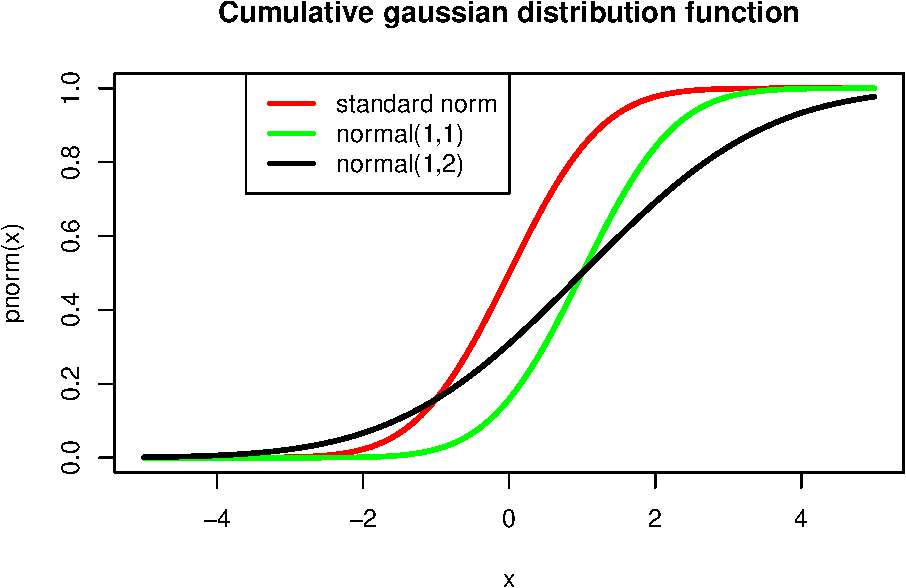
\includegraphics{probability_files/figure-latex/unnamed-chunk-18-1.pdf}

\begin{Shaded}
\begin{Highlighting}[]
\CommentTok{#density}
\KeywordTok{curve}\NormalTok{(}\KeywordTok{dnorm}\NormalTok{(x), }\DataTypeTok{xlim=}\KeywordTok{c}\NormalTok{(-}\DecValTok{5}\NormalTok{,}\DecValTok{5}\NormalTok{), }\DataTypeTok{col=}\StringTok{'red'}\NormalTok{, }\DataTypeTok{lwd=}\DecValTok{3}\NormalTok{)}
\KeywordTok{curve}\NormalTok{(}\KeywordTok{dnorm}\NormalTok{(x,}\DecValTok{1}\NormalTok{,}\DecValTok{1}\NormalTok{), }\DataTypeTok{add=}\NormalTok{T, }\DataTypeTok{col=}\StringTok{'green'}\NormalTok{, }\DataTypeTok{lty=}\DecValTok{2}\NormalTok{, }\DataTypeTok{lwd=}\DecValTok{3}\NormalTok{)}
\KeywordTok{curve}\NormalTok{(}\KeywordTok{dnorm}\NormalTok{(x,}\DecValTok{1}\NormalTok{,}\DecValTok{2}\NormalTok{), }\DataTypeTok{add=}\NormalTok{T, }\DataTypeTok{col=}\StringTok{'black'}\NormalTok{, }\DataTypeTok{lty=}\DecValTok{3}\NormalTok{, }\DataTypeTok{lwd=}\DecValTok{3}\NormalTok{)}

\KeywordTok{legend}\NormalTok{(}\KeywordTok{par}\NormalTok{(}\StringTok{'usr'}\NormalTok{)[}\DecValTok{2}\NormalTok{], }\KeywordTok{par}\NormalTok{(}\StringTok{'usr'}\NormalTok{)[}\DecValTok{4}\NormalTok{], }\DataTypeTok{xjust=}\DecValTok{1}\NormalTok{,}
       \KeywordTok{c}\NormalTok{(}\StringTok{'standard normal'}\NormalTok{, }\StringTok{'normal(1,1)'}\NormalTok{,}\StringTok{'normal(1,2)'}\NormalTok{),}
       \DataTypeTok{lwd=}\DecValTok{2}\NormalTok{, }\DataTypeTok{lty=}\KeywordTok{c}\NormalTok{(}\DecValTok{1}\NormalTok{,}\DecValTok{2}\NormalTok{,}\DecValTok{3}\NormalTok{),}
       \DataTypeTok{col=}\KeywordTok{c}\NormalTok{(}\StringTok{'red'}\NormalTok{,}\StringTok{'green'}\NormalTok{,}\StringTok{'black'}\NormalTok{))}
\end{Highlighting}
\end{Shaded}

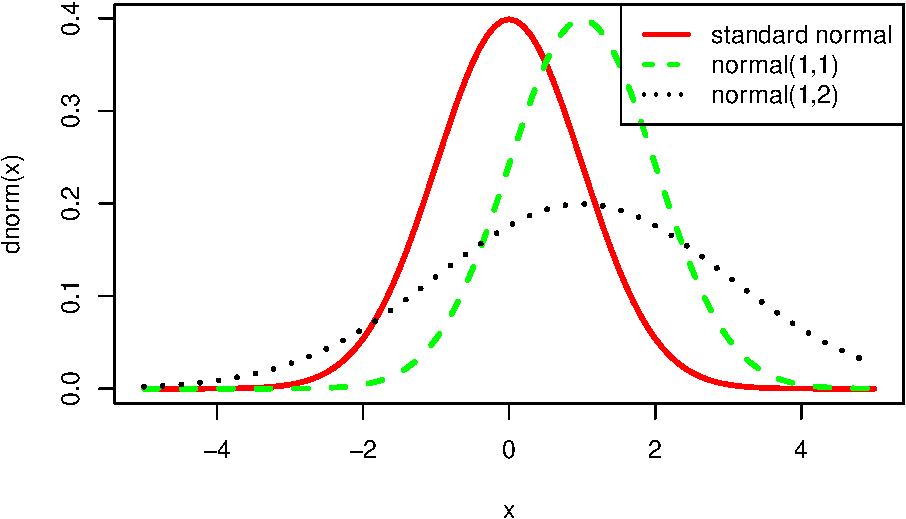
\includegraphics{probability_files/figure-latex/unnamed-chunk-18-2.pdf}

\begin{Shaded}
\begin{Highlighting}[]
\NormalTok{m <-}\StringTok{ }\KeywordTok{c}\NormalTok{(-}\DecValTok{2}\NormalTok{,}\DecValTok{0}\NormalTok{,}\DecValTok{2}\NormalTok{)    }\CommentTok{# Means}
\NormalTok{p <-}\StringTok{ }\KeywordTok{c}\NormalTok{(.}\DecValTok{3}\NormalTok{,.}\DecValTok{4}\NormalTok{,.}\DecValTok{3}\NormalTok{)  }\CommentTok{# Probabilities}
\NormalTok{s <-}\StringTok{ }\KeywordTok{c}\NormalTok{(}\DecValTok{1}\NormalTok{, }\DecValTok{1}\NormalTok{, }\DecValTok{1}\NormalTok{)   }\CommentTok{# Standard deviations}
 
\KeywordTok{curve}\NormalTok{(p[}\DecValTok{2}\NormalTok{]*}\KeywordTok{dnorm}\NormalTok{(x, }\DataTypeTok{mean=}\NormalTok{m[}\DecValTok{2}\NormalTok{], }\DataTypeTok{sd=}\NormalTok{s[}\DecValTok{2}\NormalTok{]),}
      \DataTypeTok{col =} \StringTok{"green"}\NormalTok{, }\DataTypeTok{lwd =} \DecValTok{3}\NormalTok{, }
      \DataTypeTok{xlim =} \KeywordTok{c}\NormalTok{(-}\DecValTok{5}\NormalTok{,}\DecValTok{5}\NormalTok{),}\DataTypeTok{ylim=}\KeywordTok{c}\NormalTok{(}\DecValTok{0}\NormalTok{,}\FloatTok{0.23}\NormalTok{),}
      \DataTypeTok{main =} \StringTok{"The three gaussian distributions in our mixture"}\NormalTok{,}
      \DataTypeTok{xlab =} \StringTok{""}\NormalTok{, }\DataTypeTok{ylab =} \StringTok{""}\NormalTok{)}
\KeywordTok{curve}\NormalTok{(p[}\DecValTok{1}\NormalTok{]*}\KeywordTok{dnorm}\NormalTok{(x, }\DataTypeTok{mean=}\NormalTok{m[}\DecValTok{1}\NormalTok{], }\DataTypeTok{sd=}\NormalTok{s[}\DecValTok{1}\NormalTok{]),}
      \DataTypeTok{col=}\StringTok{"red"}\NormalTok{, }\DataTypeTok{lwd=}\DecValTok{3}\NormalTok{, }\DataTypeTok{add=}\OtherTok{TRUE}\NormalTok{)}
\KeywordTok{curve}\NormalTok{(p[}\DecValTok{3}\NormalTok{]*}\KeywordTok{dnorm}\NormalTok{(x, }\DataTypeTok{mean=}\NormalTok{m[}\DecValTok{3}\NormalTok{], }\DataTypeTok{sd=}\NormalTok{s[}\DecValTok{3}\NormalTok{]),}
      \DataTypeTok{col=}\StringTok{"blue"}\NormalTok{, }\DataTypeTok{lwd=}\DecValTok{3}\NormalTok{, }\DataTypeTok{add=}\OtherTok{TRUE}\NormalTok{)}
\KeywordTok{curve}\NormalTok{(p[}\DecValTok{1}\NormalTok{]*}\KeywordTok{dnorm}\NormalTok{(x, }\DataTypeTok{mean=}\NormalTok{m[}\DecValTok{1}\NormalTok{], }\DataTypeTok{sd=}\NormalTok{s[}\DecValTok{1}\NormalTok{])+}
\StringTok{      }\NormalTok{p[}\DecValTok{2}\NormalTok{]*}\KeywordTok{dnorm}\NormalTok{(x, }\DataTypeTok{mean=}\NormalTok{m[}\DecValTok{2}\NormalTok{], }\DataTypeTok{sd=}\NormalTok{s[}\DecValTok{2}\NormalTok{])+}
\StringTok{      }\NormalTok{p[}\DecValTok{3}\NormalTok{]*}\KeywordTok{dnorm}\NormalTok{(x, }\DataTypeTok{mean=}\NormalTok{m[}\DecValTok{3}\NormalTok{], }\DataTypeTok{sd=}\NormalTok{s[}\DecValTok{3}\NormalTok{]),}
      \DataTypeTok{col=}\StringTok{"black"}\NormalTok{, }\DataTypeTok{lwd=}\DecValTok{3}\NormalTok{, }\DataTypeTok{add=}\OtherTok{TRUE}\NormalTok{)}
\end{Highlighting}
\end{Shaded}

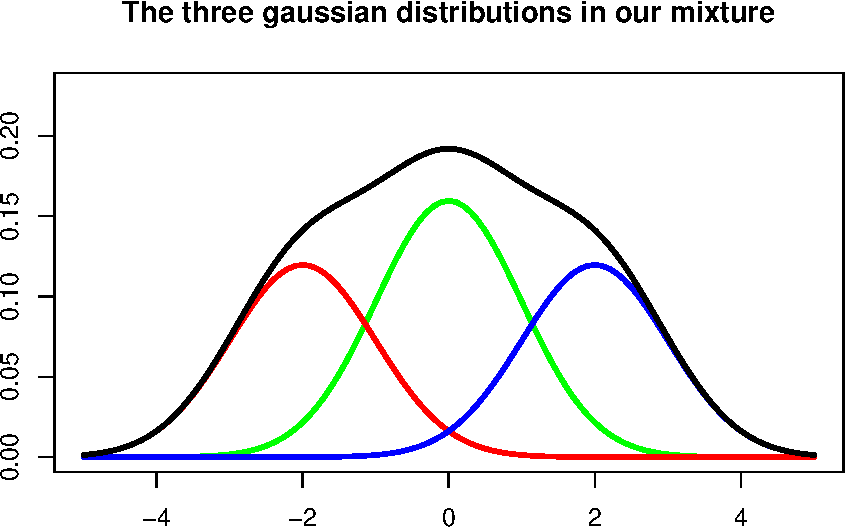
\includegraphics{probability_files/figure-latex/unnamed-chunk-19-1.pdf}

\textbf{指数分布}

\begin{Shaded}
\begin{Highlighting}[]
\KeywordTok{dexp}\NormalTok{(}\DecValTok{5}\NormalTok{, }\DataTypeTok{rate =} \DecValTok{1}\NormalTok{, }\DataTypeTok{log =} \OtherTok{FALSE}\NormalTok{)}
\end{Highlighting}
\end{Shaded}

\begin{verbatim}
## [1] 0.006737947
\end{verbatim}

\begin{Shaded}
\begin{Highlighting}[]
\KeywordTok{pexp}\NormalTok{(}\DecValTok{5}\NormalTok{, }\DataTypeTok{rate =} \DecValTok{1}\NormalTok{, }\DataTypeTok{lower.tail =} \OtherTok{TRUE}\NormalTok{, }\DataTypeTok{log.p =} \OtherTok{FALSE}\NormalTok{)}
\end{Highlighting}
\end{Shaded}

\begin{verbatim}
## [1] 0.9932621
\end{verbatim}

\begin{Shaded}
\begin{Highlighting}[]
\KeywordTok{qexp}\NormalTok{(}\DecValTok{5}\NormalTok{, }\DataTypeTok{rate =} \DecValTok{1}\NormalTok{, }\DataTypeTok{lower.tail =} \OtherTok{TRUE}\NormalTok{, }\DataTypeTok{log.p =} \OtherTok{FALSE}\NormalTok{)}
\end{Highlighting}
\end{Shaded}

\begin{verbatim}
## Warning in qexp(5, rate = 1, lower.tail = TRUE, log.p = FALSE): NaNs
## produced
\end{verbatim}

\begin{verbatim}
## [1] NaN
\end{verbatim}

\begin{Shaded}
\begin{Highlighting}[]
\KeywordTok{rexp}\NormalTok{(}\DecValTok{5}\NormalTok{, }\DataTypeTok{rate =} \DecValTok{1}\NormalTok{)}
\end{Highlighting}
\end{Shaded}

\begin{verbatim}
## [1] 0.2474990 0.4708818 0.2867484 0.2462769 1.2192623
\end{verbatim}

\begin{Shaded}
\begin{Highlighting}[]
\CommentTok{#cumulative distribution function}
\KeywordTok{curve}\NormalTok{(}\KeywordTok{pexp}\NormalTok{(x,}\DataTypeTok{rate=}\FloatTok{0.5}\NormalTok{), }\DataTypeTok{xlim=}\KeywordTok{c}\NormalTok{(}\DecValTok{0}\NormalTok{,}\DecValTok{10}\NormalTok{), }\DataTypeTok{col=}\DecValTok{1}\NormalTok{, }\DataTypeTok{lwd=}\DecValTok{3}\NormalTok{,}
      \DataTypeTok{main=}\StringTok{'Exponential Probability Distribution Function'}\NormalTok{)}
\KeywordTok{curve}\NormalTok{(}\KeywordTok{pexp}\NormalTok{(x,}\DataTypeTok{rate=}\DecValTok{1}\NormalTok{), }\DataTypeTok{xlim=}\KeywordTok{c}\NormalTok{(}\DecValTok{0}\NormalTok{,}\DecValTok{10}\NormalTok{), }\DataTypeTok{col=}\DecValTok{2}\NormalTok{, }\DataTypeTok{lwd=}\DecValTok{2}\NormalTok{, }\DataTypeTok{lty=}\DecValTok{2}\NormalTok{,}
      \DataTypeTok{add=}\NormalTok{T)}
\KeywordTok{curve}\NormalTok{(}\KeywordTok{pexp}\NormalTok{(x,}\DataTypeTok{rate=}\DecValTok{5}\NormalTok{), }\DataTypeTok{xlim=}\KeywordTok{c}\NormalTok{(}\DecValTok{0}\NormalTok{,}\DecValTok{10}\NormalTok{), }\DataTypeTok{col=}\DecValTok{3}\NormalTok{, }\DataTypeTok{lwd=}\DecValTok{2}\NormalTok{, }\DataTypeTok{lty=}\DecValTok{3}\NormalTok{,}
      \DataTypeTok{add=}\NormalTok{T)}
\KeywordTok{curve}\NormalTok{(}\KeywordTok{pexp}\NormalTok{(x,}\DataTypeTok{rate=}\DecValTok{10}\NormalTok{), }\DataTypeTok{xlim=}\KeywordTok{c}\NormalTok{(}\DecValTok{0}\NormalTok{,}\DecValTok{10}\NormalTok{), }\DataTypeTok{col=}\DecValTok{4}\NormalTok{, }\DataTypeTok{lwd=}\DecValTok{2}\NormalTok{, }\DataTypeTok{lty=}\DecValTok{4}\NormalTok{,}
      \DataTypeTok{add=}\NormalTok{T)}
\KeywordTok{legend}\NormalTok{(}\KeywordTok{par}\NormalTok{(}\StringTok{'usr'}\NormalTok{)[}\DecValTok{2}\NormalTok{], }\KeywordTok{par}\NormalTok{(}\StringTok{'usr'}\NormalTok{)[}\DecValTok{4}\NormalTok{], }\DataTypeTok{xjust=}\DecValTok{1}\NormalTok{,}
       \KeywordTok{c}\NormalTok{(}\StringTok{'rate=0.5'}\NormalTok{,}\StringTok{'rate=1'}\NormalTok{, }\StringTok{'rate=2'}\NormalTok{,}\StringTok{'rate=10'}\NormalTok{),}
       \DataTypeTok{lwd=}\DecValTok{2}\NormalTok{, }\DataTypeTok{lty=}\KeywordTok{c}\NormalTok{(}\DecValTok{1}\NormalTok{,}\DecValTok{2}\NormalTok{,}\DecValTok{3}\NormalTok{,}\DecValTok{4}\NormalTok{),}
       \DataTypeTok{col=}\DecValTok{1}\NormalTok{:}\DecValTok{4}\NormalTok{)}
\end{Highlighting}
\end{Shaded}

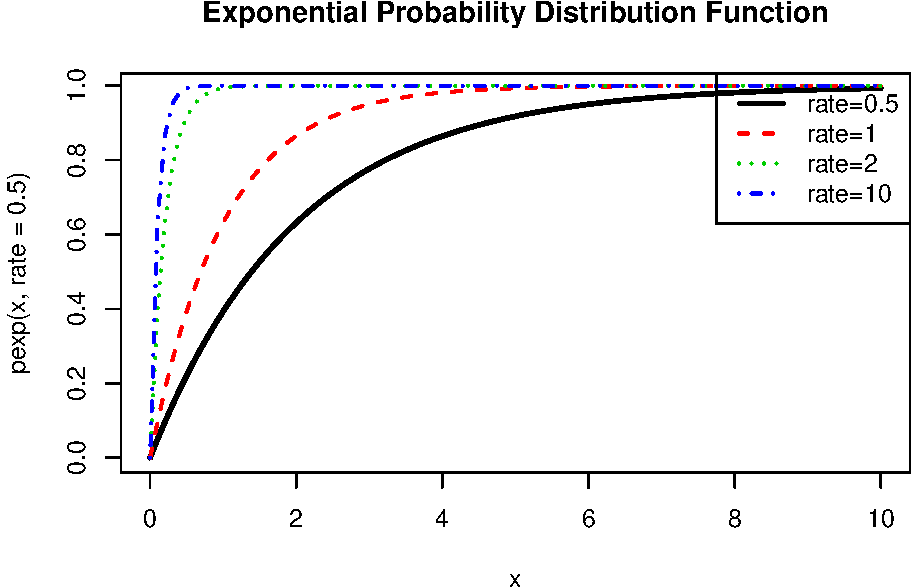
\includegraphics{probability_files/figure-latex/unnamed-chunk-21-1.pdf}

\begin{Shaded}
\begin{Highlighting}[]
\CommentTok{#density}
\KeywordTok{curve}\NormalTok{(}\KeywordTok{dexp}\NormalTok{(x,}\DataTypeTok{rate=}\FloatTok{0.5}\NormalTok{), }\DataTypeTok{xlim=}\KeywordTok{c}\NormalTok{(}\DecValTok{0}\NormalTok{,}\DecValTok{10}\NormalTok{), }\DataTypeTok{col=}\DecValTok{1}\NormalTok{, }\DataTypeTok{lwd=}\DecValTok{3}\NormalTok{,}
      \DataTypeTok{main=}\StringTok{'Exponential Probability Distribution Function'}\NormalTok{)}
\KeywordTok{curve}\NormalTok{(}\KeywordTok{dexp}\NormalTok{(x,}\DataTypeTok{rate=}\DecValTok{1}\NormalTok{), }\DataTypeTok{xlim=}\KeywordTok{c}\NormalTok{(}\DecValTok{0}\NormalTok{,}\DecValTok{10}\NormalTok{), }\DataTypeTok{col=}\DecValTok{2}\NormalTok{, }\DataTypeTok{lwd=}\DecValTok{2}\NormalTok{, }\DataTypeTok{lty=}\DecValTok{2}\NormalTok{,}
      \DataTypeTok{add=}\NormalTok{T)}
\KeywordTok{curve}\NormalTok{(}\KeywordTok{dexp}\NormalTok{(x,}\DataTypeTok{rate=}\DecValTok{5}\NormalTok{), }\DataTypeTok{xlim=}\KeywordTok{c}\NormalTok{(}\DecValTok{0}\NormalTok{,}\DecValTok{10}\NormalTok{), }\DataTypeTok{col=}\DecValTok{3}\NormalTok{, }\DataTypeTok{lwd=}\DecValTok{2}\NormalTok{, }\DataTypeTok{lty=}\DecValTok{3}\NormalTok{,}
      \DataTypeTok{add=}\NormalTok{T)}
\KeywordTok{curve}\NormalTok{(}\KeywordTok{dexp}\NormalTok{(x,}\DataTypeTok{rate=}\DecValTok{10}\NormalTok{), }\DataTypeTok{xlim=}\KeywordTok{c}\NormalTok{(}\DecValTok{0}\NormalTok{,}\DecValTok{10}\NormalTok{), }\DataTypeTok{col=}\DecValTok{4}\NormalTok{, }\DataTypeTok{lwd=}\DecValTok{2}\NormalTok{, }\DataTypeTok{lty=}\DecValTok{4}\NormalTok{,}
      \DataTypeTok{add=}\NormalTok{T)}
\KeywordTok{legend}\NormalTok{(}\KeywordTok{par}\NormalTok{(}\StringTok{'usr'}\NormalTok{)[}\DecValTok{2}\NormalTok{], }\KeywordTok{par}\NormalTok{(}\StringTok{'usr'}\NormalTok{)[}\DecValTok{4}\NormalTok{], }\DataTypeTok{xjust=}\DecValTok{1}\NormalTok{,}
       \KeywordTok{c}\NormalTok{(}\StringTok{'rate=0.5'}\NormalTok{,}\StringTok{'rate=1'}\NormalTok{, }\StringTok{'rate=2'}\NormalTok{,}\StringTok{'rate=10'}\NormalTok{),}
       \DataTypeTok{lwd=}\DecValTok{2}\NormalTok{, }\DataTypeTok{lty=}\DecValTok{1}\NormalTok{:}\DecValTok{4}\NormalTok{,}
       \DataTypeTok{col=}\DecValTok{1}\NormalTok{:}\DecValTok{4}\NormalTok{)}
\end{Highlighting}
\end{Shaded}

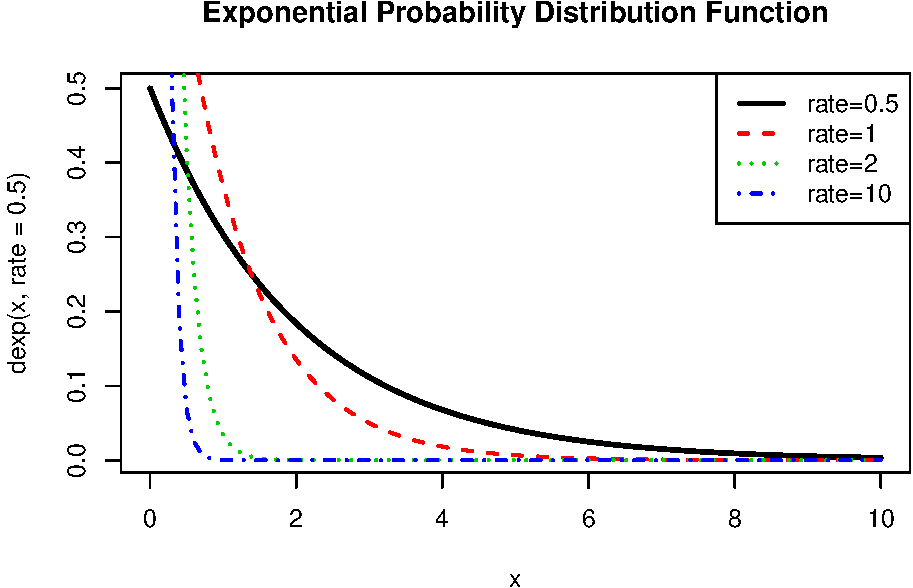
\includegraphics{probability_files/figure-latex/unnamed-chunk-21-2.pdf}

\textbf{均匀分布}

\begin{Shaded}
\begin{Highlighting}[]
\KeywordTok{dunif}\NormalTok{(}\DecValTok{5}\NormalTok{, }\DataTypeTok{min=}\DecValTok{0}\NormalTok{, }\DataTypeTok{max=}\DecValTok{1}\NormalTok{, }\DataTypeTok{log =} \OtherTok{FALSE}\NormalTok{)}
\end{Highlighting}
\end{Shaded}

\begin{verbatim}
## [1] 0
\end{verbatim}

\begin{Shaded}
\begin{Highlighting}[]
\KeywordTok{punif}\NormalTok{(}\DecValTok{5}\NormalTok{, }\DataTypeTok{min=}\DecValTok{0}\NormalTok{, }\DataTypeTok{max=}\DecValTok{1}\NormalTok{, }\DataTypeTok{lower.tail =} \OtherTok{TRUE}\NormalTok{, }\DataTypeTok{log.p =} \OtherTok{FALSE}\NormalTok{)}
\end{Highlighting}
\end{Shaded}

\begin{verbatim}
## [1] 1
\end{verbatim}

\begin{Shaded}
\begin{Highlighting}[]
\KeywordTok{qunif}\NormalTok{(}\DecValTok{5}\NormalTok{, }\DataTypeTok{min=}\DecValTok{0}\NormalTok{, }\DataTypeTok{max=}\DecValTok{1}\NormalTok{, }\DataTypeTok{lower.tail =} \OtherTok{TRUE}\NormalTok{, }\DataTypeTok{log.p =} \OtherTok{FALSE}\NormalTok{)}
\end{Highlighting}
\end{Shaded}

\begin{verbatim}
## Warning in qunif(5, min = 0, max = 1, lower.tail = TRUE, log.p = FALSE):
## NaNs produced
\end{verbatim}

\begin{verbatim}
## [1] NaN
\end{verbatim}

\begin{Shaded}
\begin{Highlighting}[]
\KeywordTok{runif}\NormalTok{(}\DecValTok{5}\NormalTok{, }\DataTypeTok{min=}\DecValTok{0}\NormalTok{, }\DataTypeTok{max=}\DecValTok{1}\NormalTok{)}
\end{Highlighting}
\end{Shaded}

\begin{verbatim}
## [1] 0.8813882 0.3047841 0.2416987 0.9618491 0.7194947
\end{verbatim}

\subsection{三、大数定律和中心极限定理}

使用\textbf{animation包}演示大数定律和中心极限定理:

\begin{Shaded}
\begin{Highlighting}[]
\CommentTok{# install.packages("animation")}
\KeywordTok{library}\NormalTok{(animation)}
\end{Highlighting}
\end{Shaded}

\subsubsection{大数定律}

LLN函数:

\begin{Shaded}
\begin{Highlighting}[]
\NormalTok{lln<-function (FUN, }\DataTypeTok{pars=}\OtherTok{NULL}\NormalTok{, }\DataTypeTok{np =} \DecValTok{30}\NormalTok{, }\DataTypeTok{n =} \KeywordTok{ani.options}\NormalTok{(}\StringTok{"nmax"}\NormalTok{),}\DataTypeTok{pch =} \DecValTok{20}\NormalTok{,}\DataTypeTok{col.poly =} \StringTok{"bisque"}\NormalTok{, }\DataTypeTok{col.mu =} \StringTok{"gray"}\NormalTok{, ...) }
\NormalTok{\{    dist.name<-}\KeywordTok{deparse}\NormalTok{(}\KeywordTok{substitute}\NormalTok{(FUN))}
     \NormalTok{if(dist.name==}\StringTok{'rbinom'}\NormalTok{)\{FUN<-function(n,pars) }\KeywordTok{rbinom}\NormalTok{(n,}\DataTypeTok{size=}\NormalTok{pars[}\DecValTok{1}\NormalTok{],}\DataTypeTok{prob=}\NormalTok{pars[}\DecValTok{2}\NormalTok{]);mu<-pars[}\DecValTok{2}\NormalTok{];\}}
     \NormalTok{if(dist.name==}\StringTok{'rpois'}\NormalTok{)\{FUN<-function(n,pars) }\KeywordTok{rpois}\NormalTok{(n,}\DataTypeTok{lambda=}\NormalTok{pars);mu<-pars;\}}
     \NormalTok{if(dist.name==}\StringTok{'rnorm'}\NormalTok{)\{FUN<-function(n,pars) }\KeywordTok{rnorm}\NormalTok{(n,}\DataTypeTok{mean=}\NormalTok{pars[}\DecValTok{1}\NormalTok{],}\DataTypeTok{sd=}\NormalTok{pars[}\DecValTok{2}\NormalTok{]);mu<-pars[}\DecValTok{1}\NormalTok{];\}}
     \NormalTok{if(dist.name==}\StringTok{'rexp'}\NormalTok{)\{FUN<-function(n,pars) }\KeywordTok{rexp}\NormalTok{(n,}\DataTypeTok{rate=}\NormalTok{pars); mu<-}\DecValTok{1}\NormalTok{/pars;\}}
     \NormalTok{if(dist.name==}\StringTok{'runif'}\NormalTok{)\{FUN<-function(n,pars) }\KeywordTok{runif}\NormalTok{(n,}\DataTypeTok{min=}\NormalTok{pars[}\DecValTok{1}\NormalTok{],}\DataTypeTok{max=}\NormalTok{pars[}\DecValTok{2}\NormalTok{]);mu<-}\KeywordTok{sum}\NormalTok{(pars)/}\DecValTok{2}\NormalTok{;\}}
     \NormalTok{if(dist.name==}\StringTok{'rchisq'}\NormalTok{)\{FUN<-function(n,pars) }\KeywordTok{rchisq}\NormalTok{(n,}\DataTypeTok{df=}\NormalTok{pars);mu<-pars;\}}
    
    \NormalTok{m =}\StringTok{ }\NormalTok{x =}\StringTok{ }\OtherTok{NULL}
    \NormalTok{for (i in }\DecValTok{1}\NormalTok{:n) \{}
        \NormalTok{d =}\StringTok{ }\KeywordTok{colMeans}\NormalTok{(}\KeywordTok{matrix}\NormalTok{(}\KeywordTok{replicate}\NormalTok{(np, }\KeywordTok{FUN}\NormalTok{(i*}\DecValTok{100}\NormalTok{,pars)), i*}\DecValTok{100}\NormalTok{))}
        \NormalTok{m =}\StringTok{ }\KeywordTok{c}\NormalTok{(m, d)}
        \NormalTok{x =}\StringTok{ }\KeywordTok{rbind}\NormalTok{(x, }\KeywordTok{range}\NormalTok{(d))}
    \NormalTok{\}}
    \NormalTok{rg =}\StringTok{ }\KeywordTok{range}\NormalTok{(m)}
    \NormalTok{xax =}\StringTok{ }\KeywordTok{pretty}\NormalTok{(}\DecValTok{1}\NormalTok{:n)}
    \NormalTok{for (i in }\DecValTok{1}\NormalTok{:n) \{}
        \KeywordTok{dev.hold}\NormalTok{()}
        \KeywordTok{plot}\NormalTok{(}\DecValTok{1}\NormalTok{:n, }\DataTypeTok{ylim =} \NormalTok{rg, }\DataTypeTok{type =} \StringTok{"n"}\NormalTok{,}
             \DataTypeTok{xlab =} \KeywordTok{paste}\NormalTok{(}\StringTok{"n =100*"}\NormalTok{, i), }
             \DataTypeTok{ylab =} \KeywordTok{expression}\NormalTok{(}\KeywordTok{bar}\NormalTok{(x)), }\DataTypeTok{xaxt =} \StringTok{"n"}\NormalTok{,}\DataTypeTok{main=}\NormalTok{dist.name)}
        \KeywordTok{axis}\NormalTok{(}\DecValTok{1}\NormalTok{, xax[xax <=}\StringTok{ }\NormalTok{i])}
        \KeywordTok{polygon}\NormalTok{(}\KeywordTok{c}\NormalTok{(}\DecValTok{1}\NormalTok{:i, i:}\DecValTok{1}\NormalTok{), }\KeywordTok{c}\NormalTok{(x[}\DecValTok{1}\NormalTok{:i, }\DecValTok{1}\NormalTok{], x[i:}\DecValTok{1}\NormalTok{, }\DecValTok{2}\NormalTok{]), }
                \DataTypeTok{border =} \OtherTok{NA}\NormalTok{, }\DataTypeTok{col =} \NormalTok{col.poly)}
        \KeywordTok{points}\NormalTok{(}\KeywordTok{rep}\NormalTok{(}\DecValTok{1}\NormalTok{:i, }\DataTypeTok{each =} \NormalTok{np), m[}\DecValTok{1}\NormalTok{:(i *}\StringTok{ }\NormalTok{np)], }\DataTypeTok{pch =} \NormalTok{pch, ...)}
        \KeywordTok{abline}\NormalTok{(}\DataTypeTok{h =} \NormalTok{mu, }\DataTypeTok{col =} \NormalTok{col.mu)}
        \KeywordTok{ani.pause}\NormalTok{()}
    \NormalTok{\}}
\NormalTok{\}}
\end{Highlighting}
\end{Shaded}

演示几个分布的大数定律:

\begin{Shaded}
\begin{Highlighting}[]
\CommentTok{# #LLN for Binomial}
\CommentTok{# lln(FUN=rbinom,pars=c(1,0.5))}
\CommentTok{# }
\CommentTok{# #LLN for Poisson}
\CommentTok{# lln(FUN=rpois,pars=2)}
\CommentTok{# }
\CommentTok{# #LLN for Uniform}
\CommentTok{# lln(FUN=runif,pars=c(0,1))}
\CommentTok{# }
\CommentTok{# #LLN for Exponential}
\CommentTok{# lln(FUN=rexp,pars=2)}
\end{Highlighting}
\end{Shaded}

\subsubsection{中心极限定理}

CLT函数:

\begin{Shaded}
\begin{Highlighting}[]
\NormalTok{clt <-}\StringTok{ }\NormalTok{function (}\DataTypeTok{obs =} \DecValTok{300}\NormalTok{, }\DataTypeTok{FUN =}\NormalTok{rexp, }\DataTypeTok{mu=}\DecValTok{0}\NormalTok{,}\DataTypeTok{sds=}\DecValTok{1}\NormalTok{,}
                 \DataTypeTok{nmax =} \KeywordTok{ani.options}\NormalTok{(}\StringTok{"nmax"}\NormalTok{),}
                 \DataTypeTok{col =} \KeywordTok{c}\NormalTok{(}\StringTok{"bisque"}\NormalTok{, }\StringTok{"red"}\NormalTok{, }\StringTok{"blue"}\NormalTok{, }\StringTok{"black"}\NormalTok{),xlim, ...) }
\NormalTok{\{}
    \NormalTok{x =}\StringTok{ }\KeywordTok{matrix}\NormalTok{(}\DataTypeTok{nrow =} \NormalTok{nmax, }\DataTypeTok{ncol =} \NormalTok{obs)}
    \NormalTok{for (i in }\DecValTok{1}\NormalTok{:nmax) x[i, ] =}\StringTok{ }\KeywordTok{apply}\NormalTok{(}\KeywordTok{matrix}\NormalTok{(}\KeywordTok{replicate}\NormalTok{(obs, }\KeywordTok{FUN}\NormalTok{(i)), i), }\DecValTok{2}\NormalTok{, mean)}
    \NormalTok{if (}\KeywordTok{missing}\NormalTok{(xlim)) xlim =}\StringTok{ }\KeywordTok{quantile}\NormalTok{(x, }\KeywordTok{c}\NormalTok{(}\FloatTok{0.005}\NormalTok{, }\FloatTok{0.995}\NormalTok{))}
    \NormalTok{for (i in }\DecValTok{1}\NormalTok{:nmax) \{}
        \KeywordTok{dev.hold}\NormalTok{()}
        \KeywordTok{hist}\NormalTok{(x[i, ], }\DataTypeTok{freq =} \OtherTok{FALSE}\NormalTok{, }\DataTypeTok{main =} \StringTok{""}\NormalTok{, }
             \DataTypeTok{xlab =} \KeywordTok{substitute}\NormalTok{(}\KeywordTok{italic}\NormalTok{(}\KeywordTok{bar}\NormalTok{(x)[i]), }\KeywordTok{list}\NormalTok{(}\DataTypeTok{i =} \NormalTok{i)), }
             \DataTypeTok{col =} \NormalTok{col[}\DecValTok{1}\NormalTok{], }\DataTypeTok{xlim =} \NormalTok{xlim)}
        \KeywordTok{lines}\NormalTok{(}\KeywordTok{density}\NormalTok{(x[i, ]), }\DataTypeTok{col =} \NormalTok{col[}\DecValTok{2}\NormalTok{],}\DataTypeTok{lwd=}\DecValTok{2}\NormalTok{)}
    \NormalTok{if(!}\KeywordTok{is.na}\NormalTok{(mu) &&}\StringTok{ }\NormalTok{!}\KeywordTok{is.na}\NormalTok{(sds))}
       \KeywordTok{curve}\NormalTok{(}\KeywordTok{dnorm}\NormalTok{(x, mu, sds/}\KeywordTok{sqrt}\NormalTok{(i)), }\DataTypeTok{col =} \NormalTok{col[}\DecValTok{3}\NormalTok{], }
             \DataTypeTok{lty =} \DecValTok{2}\NormalTok{, }\DataTypeTok{lwd=}\DecValTok{2}\NormalTok{, }\DataTypeTok{add =} \OtherTok{TRUE}\NormalTok{)}
    \KeywordTok{legend}\NormalTok{(}\StringTok{"topright"}\NormalTok{, }\DataTypeTok{legend =} \KeywordTok{c}\NormalTok{(}\StringTok{"Normal"}\NormalTok{,}\StringTok{"Est. pdf"}\NormalTok{),}
           \DataTypeTok{lty=}\DecValTok{2}\NormalTok{:}\DecValTok{1}\NormalTok{, }\DataTypeTok{lwd=}\DecValTok{2}\NormalTok{, }\DataTypeTok{col=}\KeywordTok{c}\NormalTok{(col[}\DecValTok{3}\NormalTok{],col[}\DecValTok{2}\NormalTok{]), }\DataTypeTok{bty =} \StringTok{"n"}\NormalTok{)}
    \KeywordTok{ani.pause}\NormalTok{()}
    \NormalTok{\}}
\NormalTok{\}}

\KeywordTok{ani.options}\NormalTok{(}\DataTypeTok{interval =} \FloatTok{0.5}\NormalTok{)}
\KeywordTok{par}\NormalTok{(}\DataTypeTok{mar =} \KeywordTok{c}\NormalTok{(}\DecValTok{3}\NormalTok{, }\DecValTok{3}\NormalTok{, }\DecValTok{1}\NormalTok{, }\FloatTok{0.5}\NormalTok{), }\DataTypeTok{mgp =} \KeywordTok{c}\NormalTok{(}\FloatTok{1.5}\NormalTok{, }\FloatTok{0.5}\NormalTok{, }\DecValTok{0}\NormalTok{), }\DataTypeTok{tcl =} \NormalTok{-}\FloatTok{0.3}\NormalTok{)}
\end{Highlighting}
\end{Shaded}

演示几个分布的中心极限定理:

\begin{Shaded}
\begin{Highlighting}[]
\CommentTok{# #Poisson case}
\CommentTok{#   f<-function(n) rpois(n,lambda=4);}
\CommentTok{#   clt(FUN = f, mu=4,sds=2)}
\CommentTok{# }
\CommentTok{# #binomial case}
\CommentTok{#   f<-function(n) rbinom(n,size=1,prob=0.5)}
\CommentTok{#   clt(FUN = f, mu=0.5, sds=0.5)}
\CommentTok{# }
\CommentTok{# #exponential distribution case}
\CommentTok{#   f<-function(n) rexp(n,rate=2);}
\CommentTok{#   clt(FUN = f, mu=1/2,sds=1/2)}
\CommentTok{# }
\CommentTok{# #uniform distribution case}
\CommentTok{#    f<-function(n,pars) runif(n,min=0,max=1);}
\CommentTok{#    clt(FUN = f,mu=1/2,sd=1/sqrt(12))}
\CommentTok{# }
\CommentTok{# #chi-square distribution}
\CommentTok{#   f<-function(n) rchisq(n,df=2);}
\CommentTok{#   clt(FUN = f,mu=2,sd=2)}
\end{Highlighting}
\end{Shaded}


\end{document}
